\cotefile{138}
\scanpage{90}
% archive foliation: 89
Considérons $L_\nu=\{\lambda_0,\ldots,\lambda_\nu\mid\lambda_0\lambda_1\cdots\lambda_\nu=1\}$ \unsure{groupe discret}.
\[
\unsure{\Phi_i}\in\operatorname{Homext}(\mathbb Z,L_\nu)\quad\text{classe de}
\qquad\psi_i:\mathbb Z\longrightarrow L_\nu\qquad\psi_i(1)=\lambda_i
\]
(\unsure{donc} $\Phi_i\unsure{=|:}\widehat{\psi_i}$) $\deleted{\unsure{\Phi_i=}}$

Considérons $B_\nu=\operatorname{Aut}(L_\nu,\mathbb Z,(\unsure{\Phi_i|\Psi_i}))$.

On a
\[
B_\nu\xrightarrow{\chi_\nu^\circ}\mathbb Z^*=\{\pm1\}\quad\text{surjectif}
\]
\[
L_\nu\hookrightarrow\operatorname{Ker}(\chi_\nu^\circ)\qquad g\longmapsto(\operatorname{int}(g),\operatorname{id}_{\mathbb Z}).
\]
Soit $\mathcal T_\nu=B_\nu/L_\nu$
\[
1\;\unsure{-|\longrightarrow}\;\mathcal T_\nu^\circ\longrightarrow\mathcal T_\nu\longrightarrow\mathbb Z_{/2}\longrightarrow1
\]
(\unsure{groupe de Teichmüller} (discret) non orienté pour la sphère à $\nu+1$ trous)

On sait que $\mathcal T_2^\circ=1$
\[
\mathcal T_\nu^\circ=\text{groupe des tresses sphériques coloriées à $(\nu+1)$ brins, groupe non trivial}
\quad\inserted{\text{si }\nu\geq3}\quad
[\simeq\pi_1(\widetilde D_{\nu+1})\unsure{/\mathbb Z_2}]
\]
On a
\diagram{\begin{tikzcd}
\widehat L_\nu\arrow[r,hook]\arrow[d,Rightarrow] & \widehat B_\nu\arrow[d,hook,no head]\arrow[r,"\widehat\chi_\nu^\circ"] & (\mathbb Z^*)^{\wedge}=\pm1\arrow[d,hook,no head]\\
\widehat L_\nu\arrow[r] & A_\nu\arrow[r,"\chi_\nu"] & \unsure{\mathbb Z^*|\widehat{\mathbb Z}^{*}}
\end{tikzcd}}
\[
\overline B_\nu/\widehat L_\nu=\widehat{\mathcal T}_\nu\subset A_\nu/\widehat L_\nu=\Gamma_\nu
\]
\diagram{\begin{tikzcd}
1\arrow[r] & \widehat{\mathcal T}_\nu^\circ\arrow[r,hook]\arrow[d,hook,"\unsure{\mathrm{cont}}"'] & \widehat{\mathcal T}_\nu\arrow[r]\arrow[d,hook] & \mathbb Z_{/2}\arrow[r,dash]\arrow[d,hook] &1\\
1\arrow[r] & \Gamma_\nu^\circ\arrow[r] & \Gamma_\nu\arrow[r] & \widehat{\mathbb Z}^{*}\arrow[r,dash] &1
\end{tikzcd}}
\uline{Questions} $\widehat{\mathcal T}_\nu$ invariant dans $\Gamma_\nu$? $\widehat{\mathcal T}_\nu^\circ$ \unsure{dist. ds} $\Gamma_\nu^\circ$?

Quand a-t-on \deleted{\illegible{2}} $\widehat{\mathcal T}_\nu^\circ=\Gamma_\nu^\circ$

\inserted{c'est \uline{faux} pour $\nu=2$}

\scanpage{91}
% archive foliation: 90
\uline{Variante} Donnons-nous $\varepsilon=(\varepsilon_0,\varepsilon_1,\ldots,\varepsilon_\nu)\in(\unsure{\overline{\mathbb N}^{*}|\mathbb N^{*}})^{\nu+1}$\inserted{$[1,\infty]$}.

Soit
\[
L_\nu^\varepsilon=\{\lambda_0,\ldots,\lambda_\nu\mid\lambda_0\lambda_1\cdots\lambda_\nu=\lambda_0^{\varepsilon_0}=\lambda_1^{\varepsilon_1}=\cdots=\lambda_\nu^{\varepsilon_\nu}=1\}.
\]

\scanpage{93}
% archive foliation: 92
\diagram{$\left\{\begin{array}{l|l}
\Gamma\ \text{groupe},\ C\ \Gamma\text{-torseur à droite}&\\
\pi,\ \Gamma\text{-groupe}\qquad\deleted{\widetilde\pi,\unsure{\text{groupe}}}&\widetilde\pi\ \text{groupe}\\
T_i\ (i\in I)\ (\pi,\Gamma)\text{-tors.}&\widetilde T_i\ (i\in I)\ \widetilde\pi\text{-torseurs}\\
\pi_i\ \unsure{\text{commutants}|\text{commutatifs}}&\widetilde\pi_i\ \unsure{\text{les}|\text{non}}\ \unsure{\text{commutants}|\text{commutatifs}}\\
I_i\hookrightarrow\pi_i\quad\text{sous-}\Gamma\text{-groupe}&\widetilde I_i\subset\widetilde\pi_i
\end{array}\right.$}
\[
C\xrightarrow{\varphi}\operatorname{Isom}(\pi,\widetilde\pi)\qquad\Gamma\text{-homomorphisme}
\]
\deleted{$\unsure{f}\quad\rho(\varphi):\pi\unsure{-|\longrightarrow}\widetilde\pi$}
\qquad
\diagram{\begin{tikzcd}
\deleted{\pi}\arrow[r,dash,"\deleted{\rho(\varphi)}"]&\deleted{\widetilde\pi}\\
\deleted{T_i}\arrow[r,"\deleted{\rho_i(\varphi)}"]&\deleted{\widetilde T_i}
\end{tikzcd}}
\deleted{$\unsure{R}\quad T_i\wedge_\pi(\widetilde\pi,\varphi)$}
\qquad donc $\widetilde\pi\simeq C\wedge_\Gamma\pi$
\[
\left\{\begin{aligned}
\widetilde\pi&=C\wedge_\Gamma\pi\\
(\widetilde\pi_i,\widetilde T_i,\widetilde\pi)&=C\wedge_\Gamma(\pi_i,T_i,\pi)\\
\deleted{\unsure{\widetilde\pi_i}}\quad\widetilde I_i&\subset\widetilde\pi_i\qquad\widetilde I_i=C\wedge_\Gamma I_i
\end{aligned}\right.
\qquad\text{donc}\quad I_i=\unsure{\check C\wedge_\Gamma\widetilde I_i\wedge_\Gamma C}
\]
\[
\widetilde I_i\simeq\widehat{\mathbb Z}\quad\text{d'où}\quad\chi_i:\Gamma\longrightarrow\widehat{\mathbb Z}^{*}\simeq\operatorname{Aut}(I_i)
\]
\uline{\unsure{Indép. de $i$|Indép. de $\nu$}}

\scanpage{94}
% archive foliation: 93
$\Gamma\ (=\operatorname{Aut}(\overline{\mathbb Q}))$ groupe, $C$ $\Gamma$-tors. à droite
\inserted{$(=\operatorname{Isom}(\overline{\mathbb Q},\unsure{\mathbb C}))$}

$\pi\ (=\pi_1(\mathbb P^1_{\overline{\mathbb Q}}-I_{\overline{\mathbb Q}}))$ $\Gamma$-groupe
\qquad $(I\subset\mathbb P^1(\mathbb Q))$ fini

$\forall i\in I\quad T_i$ un $(\pi,\Gamma)$ torseur à droite
\qquad $(=\operatorname{Isom}(F_{\unsure{\bar\xi_\eta}},F_{\unsure{\bar\xi_i}}))$

$\forall i\quad r_i:C\longrightarrow T_i$ satisfaisant,
\[
r_i(\varphi\sigma)=\sigma^{-1}\cdot r_i(\varphi)\qquad/\quad r:C\longrightarrow\prod T_i
\]
\[
\pi_i=\operatorname{Aut}_\pi(T_i)\quad\text{commutant de $\pi$ ds $T_i$}
\]
\[
\simeq T_i\wedge_\pi(\pi\ \mathrm{int})
\]
\[
I_i\left(=\unsure{\mathrm T_{\bullet}}(\overline{\mathbb Q})\right)\hookrightarrow\pi_i
\qquad\text{hom de $\Gamma$-groupes}
\]
\[
\unsure{\mathrm T_{\bullet}}(\overline{\mathbb Q})=\varprojlim_n\mu_n(\overline{\mathbb Q})
\qquad\text{avec }I_i\simeq\widehat{\mathbb Z}\quad(\text{pro-cyclique})
\]
\diagram{\begin{tikzpicture}
\node (D) at (0,0) {$\begin{tikzcd}[column sep=huge,row sep=large]
\unsure{\mathcal C\simeq|\mathcal C=} (\pi\text{-ens})\arrow[r,dash,"f"]\arrow[d,"\overline F_i(E)=T_i\wedge_\pi E"]\arrow[dd,bend right=50,"f_i"'] & (\mathrm{ens})\\
\pi_i\text{-(ens)}\arrow[d] & E_i\longrightarrow E_i/I_i=\widetilde E_i\\
\mathrm{Ens} &
\end{tikzcd}$};
\node at (3.5,0.5) {oubli de $\pi$};
\draw (3,0.65) .. controls (2,0.9) and (2,1.5) .. (1.5,1.75);
\draw (-5.1,2.5) .. controls (-2.5,2.8) and (4.4,2.8) .. (5,1.7) .. controls (5.5,0.8) and (5.7,0) .. (5.4,-0.5) -- (-1.8,-3.2);
\end{tikzpicture}}
\[
C\;\unsure{-|\longrightarrow}\;\operatorname{Isom}(\pi,\unsure{\widetilde\pi}).
\]

\scanpage{95}
% archive foliation: 94
\diagram{\begin{tikzcd}
\pi_i\arrow[r]&\pi\\
I_i\arrow[u]\arrow[ur,"\alpha_i(\varphi)"']\arrow[d,equals]&\\
I&
\end{tikzcd}}
\[
\alpha(\varphi\gamma)(\lambda)=\gamma_\pi^{-1}\alpha(\varphi)(\overbrace{\gamma_I(\lambda)}^{\lambda^\gamma})
\]
\[
\gamma_\pi^{-1}\alpha_i(\varphi_0)(\lambda_i)=l_i
\]
\[
l_1\cdots l_n
\]
\[
\gamma_\pi^{-1}(l_1^\gamma),\ldots,\gamma_\pi^{-1}(l_n^\gamma)
\]
\[
l_1l_2\cdots l_n=1
\]
\[
\gamma_\pi^{-1}(\unsure{l_n|l_1})
\]
\par\noindent\rule{\linewidth}{0.3pt}
\[
C\xrightarrow{\rho_i}\operatorname{Isom}(\widehat{\mathbb Z},I_i)\qquad\rho_i(\varphi)(\unsure{1|u})=\lambda_i(\varphi)
\]
\[
\unsure{\pi|\Gamma}\xrightarrow{\chi}\widehat{\mathbb Z}^{*}\qquad\text{indépendant de $i$}
\]
\[
\lambda_i(\varphi\gamma)=\chi(\unsure{\sigma|\gamma})\lambda_i(\varphi)
\]
\[
\rho_i(\varphi\gamma)(n)=\rho_i(\varphi)(\deleted{\unsure{n^{\chi(\unsure{\sigma|\gamma})}}}\chi(\unsure{\sigma|\gamma})\cdot n)=\chi(\unsure{\sigma|\gamma})\rho_i(\varphi)(n)
\]
\[
\lambda_i(\varphi)\in I_i\xrightarrow{\widetilde r_i(\varphi)}\pi
\]

\scanpage{96}
% archive foliation: 95
\[
(\varphi\in C)\longmapsto\underbrace{\pi\xleftarrow[\sim]{\alpha_i(\varphi)}\pi_i}_{\substack{\text{pas compatible}\\\text{avec }\Gamma}}\quad\text{d'où}\quad I_i\subset\pi_i
\]
\[
\alpha_i(\varphi\gamma)=\gamma_\pi^{-1}\alpha_i(\varphi)\gamma_{\pi_i}
\]
\[
C\xrightarrow{\beta}\operatorname{Isom}(\pi,\widetilde\pi)\qquad\beta(\varphi\gamma)=\beta(\varphi)\cdot\gamma_\pi
\]
\diagram{\begin{tikzcd}
\pi\arrow[r,"\beta(\varphi)"]&\deleted{\unsure{t}}\ \unsure{\widetilde\pi}\\
I_i\arrow[u,"\alpha_i(\varphi)"]\arrow[ur,"\alpha'_i(\varphi)"']&
\end{tikzcd}}
\[
\begin{aligned}
\alpha'_i(\varphi\gamma)&=\beta(\varphi\gamma)\alpha_i(\varphi\gamma)=\beta(\varphi)\gamma_\pi\gamma_\pi^{-1}\alpha_i(\varphi)\gamma_{\pi_i}\\
&=\beta(\varphi)\alpha_i(\varphi)\gamma_{\pi_i}=\alpha'_i(\varphi)\gamma_{\pi_i}.
\end{aligned}
\]
donc $\widetilde I_i=\alpha'_i(\varphi)(I_i)$ indépendant de $\unsure{i|\varphi}$
\[
\deleted{\operatorname{Isom}(I_i,\widetilde I_i)}=\qquad\widetilde I_i=C\wedge_\pi I_i
\]
\unsure{Si|$l_i$}\quad $\deleted{\unsure{\pi_i}=\pi/\unsure{H_i};\unsure{H_i}}$
\quad $\pi'_i=\pi/N_i$\quad $N_i=$ sous-groupe de $\pi$ opérant trivialement sur $I_i$ (indépendt de $i$)
\[
\widetilde I_i=C\wedge_\pi I_i
\]
\[
I_i\simeq\unsure{\mathrm T_{\bullet}}(\overline{\mathbb Q})\qquad\pi'\simeq\operatorname{Aut}(I_i)\simeq\widehat{\mathbb Z}^{*}
\]
\[
C\simeq\varprojlim\mu_n(\overline{\mathbb Q})^{*}
\]

\scanpage{97}
% archive foliation: 96
\margin{\unsure{précartes} et cartes \unsure{tot$^t$|de $h^+$}\\
\unsure{épinglées} \unsure{par|pour}\\
précartes\ldots}

\scanpage{98}
% archive foliation: 97
% A faint upper-right mark resembles 1; not securely distinguishable from later foliation.
Cartes \inserted{\uline{totalement}} épinglées. etc.

I) Appelons pré-carte un système $(S,A,F\deleted{\unsure{\}}};p,q,r)$ où $S,A,F$ sont des ensembles, $p,q,r$ des applications
\deleted{de $S,A,$}
\[
S\xrightarrow{p}\mathbb N^{*}\qquad A\xrightarrow{q}\mathbb N^{*}\qquad F\xrightarrow{r}\mathbb N^{*}
\]
et $q$ ne prenant que les valeurs $1$ et $2$.

\unsure{Ils|Il} forment une catégorie pour les \deleted{iso.}\inserted{morphismes} $\varphi$ de $(S',A',F';p',q',r')\longrightarrow(S,A,F,p,q,r)$
\deleted{(\unsure{cartes}) \unsure{triples} d'}
\deleted{À toute carte combinatoire $C$, on associe \unsure{une pré-carte}}
\inserted{applications}
\deleted{$\varphi_s:S'\;\unsure{-|\longrightarrow}\;S$}
\[
\varphi_s:S'\longrightarrow S,\quad\varphi_a:A'\;\unsure{-|\longrightarrow}\;A,\quad\varphi_f:F'\;\unsure{-|\longrightarrow}\;F
\]
satisfaisant
\[
\left\{\begin{aligned}
&\deleted{p(\varphi_s(s'))\mid p'(\unsure{s'})}\quad\inserted{p'(s')=\nu(\varphi,s)\,p(s)}
&&\forall s'\in S',\ s=\varphi_s(s')\\
&\deleted{q(\varphi_a(a'))\mid q'(\unsure{a'})}\quad\inserted{q'(a')=\nu(\varphi,a)\,q(a)}
&&\forall a'\in A',\ a=\varphi_a(a')\\
&\deleted{r(\varphi_f(f'))\mid r'(\unsure{f'})}\quad\inserted{r'(f')=\nu(\varphi,\unsure{f|r})\,r(f)}
&&\forall f'\in F',\ f=\varphi_f(f')
\end{aligned}\right.
\]
où $\nu(\varphi,s)=\operatorname{Card}(\varphi_s^{-1}(s))$, $\nu(\varphi,a)=\text{---}$, $\nu(\varphi,f)=\text{---}$.

On a un foncteur évident de la catégorie \inserted{$(\mathrm{Cartcomb})$} des cartes comb. (avec bords, \inserted{\unsure{facettes pendantes}} \unsure{plis}) dans celle des précartes, $(\mathrm{Précart})$,
\[
C\longmapsto\operatorname{Fac}(C).
\]
\deleted{Appelons épinglage d'}
Ce foncteur est conservatif\margin{$\operatorname{Fac}(u)$ iso $\Rightarrow u$ iso}.
\margin{\unsure{D'où} \uline{\unsure{fidèle}}\quad \unsure{ce foncteur est} \unsure{fidèle} pour iso}

Soit $\mathcal C_0=(S,A,F,p,q,r)$ une pré-carte.
On appelle carte \inserted{comb.} $\mathcal C_0$-épinglée la donnée d'une carte $C$ et d'un iso.
\[
\deleted{\unsure{\operatorname{Fac}(C)}\longrightarrow\unsure{C}}
\qquad\mathcal C_0\xrightarrow[\sim]{u}\operatorname{Fac}(C)
\]
\deleted{\unsure{C'est une}} Les morphismes sont les morphismes de cartes compatibles avec l'épinglage $\mathcal C_0$, bien sûr des isomo. de cartes, et il se

\scanpage{99}
% archive foliation: 98
trouve que la catégorie des cartes \inserted{\uline{orientées}} $\mathcal C_0$-épinglées est rigide -- donc équivalente à une catégorie discrète. \deleted{\unsure{Donc}} Dans le cas où $\mathcal C_0$ est fini, cette catégorie est \unsure{elle} $\simeq$ finie. Elle est vide sauf si
\[
\sum_s p(s)=\sum_a q(a)=\sum_f r(f),
\]
et si cette condition est vérifiée, soit \deleted{$\unsure{d}$}\inserted{$\delta$} la \deleted{\unsure{valeur}}\inserted{valeur} commune des trois -- alors le \deleted{\unsure{nombre des}}\inserted{cardinal de l'} classes d'isomorphie des $\mathcal C_0$-cartes est égal à \unsure{l'ens.} des classes d'iso. de $\mathcal G_2^\circ$-ens $E$ ``admissibles'' de cardinal $\delta$, ayant les \unsure{mêmes} \deleted{\unsure{invariants}} nombres de multiplicité que $\mathcal C_0$, \uline{multiplié} par le cardinal du groupe des autom. de $\mathcal C_0$, qui est égal à
\[
\prod_{n\in\mathbb N^*}(a_n!\,b_n!\,c_n!)
\]
où $a_n(b_n,c_n)$ est le nb de sommets (arêtes, faces) de degré $n$.

\margin{Définir ici $C_{\mathcal C_0}$ et $C_{\mathcal C_0}^{\alpha}$, et l'opération de $\gamma=\gamma_{\mathcal C_0}=\operatorname{Aut}(\mathcal C_0)$ dessus. -- \uline{NB} $C_{\mathcal C_0}^{\alpha}/\gamma\;\unsure{-|\longrightarrow}\;$ l'ens des classes d'iso. de cartes de type $(\mathcal C_0,\alpha)$\ldots}

\scanpage{100}
% archive foliation: 99
II) Supposons $\mathcal C_0$ fini. Pour un schéma de base $T$,

\deleted{Appelons revêtement spécial $\mathcal C_0$-épinglé de $\mathbb P^1_T$, un rev. fini \inserted{$X\xrightarrow{f}\mathbb P^1_T$} de $\mathbb P^1_T$, étale sur $U_T=\mathbb P^1_T-\{0,1,\infty\}$, avec \deleted{\unsure{une}}\inserted{ramification} modérée fibre par fibre, et \deleted{des \illegible{1}}\inserted{isomorphismes}}
\[
\deleted{f^{-1}(0_T)_{\unsure{\mathrm{red}}}\simeq}
\]
\[
\begin{aligned}
f^{-1}(0_T)_{\mathrm{réd}}&\simeq\deleted{\unsure{T}}\ S_{T\,\deleted{\unsure{\mathrm{ét}}}\,\mathrm{réd}}\\
f^{-1}(1_T)_{\mathrm{réd}}&\simeq A_{T\,\deleted{\unsure{\mathrm{ét}}}\,\mathrm{réd}}\\
f^{-1}(\infty_T)_{\mathrm{réd}}&\simeq F_{T\,\deleted{\unsure{\mathrm{réd}}}}
\end{aligned}
\]
\deleted{qui fibre par fibre sont \unsure{des isom.} \unsure{précisés} par}
\inserted{``compatibles avec les degrés de ramification'' $(p,q,r,\ \text{en bas})$}
\margin{\deleted{\unsure{fibre par fibre}\ \unsure{évidente}\ \unsure{isomorphismes}\ \unsure{aux fibres}\ \unsure{uniforme}}}

\deleted{\unsure{De plus}} On voit que \deleted{cette} catégorie est rigide.\margin{vérifier}
\deleted{Pour $\mathcal C_0$ fini,} Soit \deleted{$\unsure{F}$} $P_{\mathcal C_0}(S)$ l'ens des classes d'iso. de cette catégorie. On voit que pour $S$ variable, on a un foncteur contravariant en $S$, qui est représentable. On trouve que le schéma $M_{\mathcal C_0}$ qui le représente est quasi fini, \deleted{et} étale et séparé sur $\mathbb Z$; il est de plus \uline{fini} au dessus de $\mathbb Z[\frac1{\delta!}]$ -- i.e. aux voisinages en car. $p>\delta$ ($\delta=$ complexité de $\mathcal C_0$)

\scanpage{101}
% archive foliation: 100
On s'intéresse surtout au schéma $(M_{\mathcal C_0})_{\mathbb Q}$ --- qui est donc fini étale sur $\mathbb Q$, non ramifié en les $p>\delta$.

\deleted{\unsure{Sur ce schéma}}
\deleted{Je \unsure{le désignerai}}

Sur le schéma $M_{\mathcal C_0}$, le gr. $\gamma_{\mathcal C_0}=\operatorname{Aut}(\mathcal C_0)$ opère de façon évidente car il opère sur $F_{\mathcal C_0}$. Le stabilisateur d'une section de $M_{\mathcal C_0}$ sur un $T$, i.e. d'une classe d'iso de ) $X\xrightarrow{f}\mathbb P^1_S$ \unsure{\ldots} avec \deleted{$\unsure{\gamma}$} $\mathcal C_0$-\deleted{\unsure{ori}}épinglage, correspond \inserted{(si $S$ est connexe)} aux autom du \deleted{$X\unsure{-f}$} rev. $X\xrightarrow{f}\mathbb P^1_S$ indépendamment de l'épinglage. P. ex. si $f$ est galoisien, il est can. iso. au groupe de Galois de $f$.

Pour.\ $\unsure{\forall}$ classe d'iso. $\alpha$ de \deleted{cartes}\inserted{groupes} \deleted{(non épinglées)} \inserted{finis}, \deleted{orientées (de type $\mathcal C_0$)} \inserted{\unsure{(constant fini)}} soit $F_{\mathcal C_0}^{\alpha}$ le sous-foncteur \deleted{que} $F_{\mathcal C_0}$ qui correspond aux $X\xrightarrow{f}\mathbb P^1_T$ tels que sur \inserted{chaque} fibre géom., le groupe de Galois du

\scanpage{102}
% archive foliation: 101
rev. étale galoisien \inserted{de $\mathbb P^1_T$} engendré par $f$ est de type $\alpha$. Il est évidemment stable par $\gamma_{\mathcal C_0}$, et correspond à un sous-\deleted{foncteur}\inserted{schéma} ouvert et fermé $M_{\mathcal C_0}^{\alpha}$ de $M_{\mathcal C_0}$, stable par $\gamma_{\mathcal C_0}$.

[Il est vide sauf si le cardinal $N$ de $\alpha$ est un multiple commun des $p(s),q(s),r(s)$ et de $\delta$; \deleted{$\unsure{\exists}$} et $M$ est non vide ssi \deleted{$\exists$} $G$ \inserted{de type $\alpha$} est engendrable par des gén.\ \deleted{$\unsure{k,l}$} $\rho_s,\inserted{\sigma,}\rho_f$ satisfaisant $\rho_s\rho_f\sigma=1$, $\sigma^2=1$, et si \deleted{$\unsure{\forall}$} $\exists\ H$ ss-groupe de $G$, avec $\bigcap\text{conjugués de }H=\{e\}$, et $\mathcal C_0$ déduit de la carte combinatoire orientée $E=G/H$ avec les \unsure{op.}\ $\rho_s,\rho_f,\sigma$ \unsure{opérant dessus}]. Mais il est important de réaliser que \unsure{lors même} qu'on aurait $N=\delta$ i.e.\ $H=\{e\}$, la classe d'isom. de $G$ \uline{muni de} $\rho_s,\rho_f,\sigma$ (i.e. le type de carte combinatoire orientée correspondante) \uline{n'est pas} déterminée par la seule connaissance de $X\xrightarrow{f}\mathbb P^1_{\mathbb C}$\ldots]

\scanpage{103}
% archive foliation: 102
\uline{III}) Conclusion, \inserted{$M^{\alpha}_{\mathcal C_0}(\overline{\mathbb Q})\simeq$} $M^{\alpha}_{\mathcal C_0}(\mathbb C)$ [$=M^{\alpha}_{\mathcal C_0\mathbb Q}(\mathbb C)\simeq\operatorname{Hom}(R^{\alpha}_{\mathcal C_0},\mathbb C)$, où $R^{\alpha}_{\mathcal C_0}$ est l'algèbre finie étale sur $\mathbb Q$ qui représente $M^{\alpha}_{\mathcal C_0\mathbb Q}$].
\margin{$\overline{\mathbb Q}=$ clôture alg. de $\mathbb Q$ dans $\mathbb C$}

On sait que c'est aussi l'ens $C^{\alpha}_{\mathcal C_0}$ des \inserted{classes d'iso} cartes \inserted{comb.} orientées qui sont de type $(\mathcal C_0,\alpha)$, i.e. Donc $\Gamma=\operatorname{Aut}(\overline{\mathbb Q})$ opère dans $\unsure{C}^{\alpha}_{\mathcal C_0}$ --- en fait \unsure{la} \deleted{l'opération}\inserted{connaissance} du $\Gamma$-ens \deleted{\unsure{i.e. op.}} $C^{\alpha}_{\mathcal C_0}$ signifie \deleted{\unsure{(à}} la conn. (à iso can. près) du $\mathbb Q$-schéma $M^{\alpha}_{\mathcal C_0\mathbb Q}$ (ou du $\mathbb Z[\frac1{\delta!}]$-schéma $(M^{\alpha}_{\mathcal C_0})_{\mathbb Z[\frac1{\delta!}]}$ \ldots). Bien entendu, $\Gamma$ opère de façon compatible \inserted{(i.e. commutant)} avec les opérations de $\gamma$ sur $C^{\alpha}_{\mathcal C_0}$.

Rien qu'en regardant l'élém. $\tau$ de $\Gamma$, $\tau z=\bar z$, on voit que l'opération de $\Gamma$ sur $C^{\alpha}_{\mathcal C_0}/\gamma$ peut ne pas être triviale\ldots

On va essayer de déterminer l'opération de $\gamma\times\Gamma$ sur $C^{\alpha}_{\mathcal C_0}$ dans certains cas élémentaires (cartes sphériques\ldots)

\scanpage{104}
% archive foliation: 103
\textcircled{1} Carte combinatoire \uline{type}
\figure{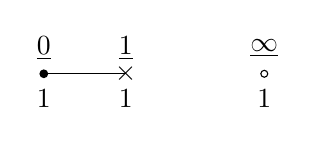
\begin{tikzpicture}[scale=.8]
\draw (0,0)--(1.3,0);\fill (0,0) circle(.07);\node at(1.3,0){$\times$};
\node at(0,.4){$\underline0$};\node at(1.3,.4){$\underline1$};\node at(0,-.4){$1$};\node at(1.3,-.4){$1$};
\draw(3.5,0)circle(.055);\node at(3.5,.4){$\underline\infty$};\node at(3.5,-.4){$1$};
\end{tikzpicture}}
$G\xrightarrow{\sim}\unsure{\gamma}\simeq1\quad\unsure{\delta}=1$
\deleted{$\gamma\simeq\{1\}$}
\margin{$1\quad1\quad1$}
\[f(z)=z\]

\textcircled{2} Carte combinatoire type
\figure{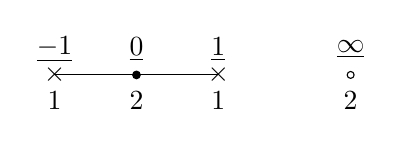
\begin{tikzpicture}[scale=.8]
\draw(-1.3,0)--(1.3,0);\node at(-1.3,0){$\times$};\fill(0,0)circle(.07);\node at(1.3,0){$\times$};
\node at(-1.3,.4){$\underline{-1}$};\node at(0,.4){$\underline0$};\node at(1.3,.4){$\underline1$};
\node at(-1.3,-.4){$1$};\node at(0,-.4){$2$};\node at(1.3,-.4){$1$};\draw(3.4,0)circle(.055);\node at(3.4,.4){$\underline\infty$};\node at(3.4,-.4){$2$};
\end{tikzpicture}}
$G\xrightarrow{\sim}\unsure{\gamma}\simeq\mathbb Z_2\quad\unsure{\delta}=2$
\deleted{$\gamma\simeq\mathbb Z_2$}
\margin{$\begin{array}{ccc}&1&\\2&&2\\&1&\end{array}$}
\[f(z)=z^2\qquad C_{\mathcal C_0}=C^{\alpha}_{\mathcal C_0}\text{ n'a qu'un élément}\ \deleted{\unsure{a}}\]

\textcircled{$2'$} Carte comb. type
\figure{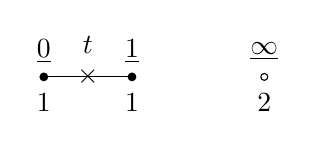
\begin{tikzpicture}[scale=.8]
\draw(0,0)--(1.4,0);\fill(0,0)circle(.07);\node at(.7,0){$\times$};\fill(1.4,0)circle(.07);
\node at(0,.4){$\underline0$};\node at(.7,.5){$\unsure{t}$};\node at(1.4,.4){$\underline1$};\node at(0,-.4){$1$};\node at(1.4,-.4){$1$};\draw(3.5,0)circle(.055);\node at(3.5,.4){$\underline\infty$};\node at(3.5,-.4){$2$};
\end{tikzpicture}}
$G\xrightarrow{\sim}\unsure{\gamma}\simeq\mathbb Z_2\quad\unsure{\delta}=2$
\deleted{$\gamma\simeq\mathbb Z_2$}
\margin{$\begin{array}{ccc}1&&\\&2&2\\1&&\end{array}$}
\[
\left[f(z)=\lambda z(z-1)\qquad
\left\{\begin{array}{l}f(t)=\lambda t(t-1)=1\\f'(t)=\lambda(2t-1)=0\end{array}\right.
\quad\deleted{\unsure{t}}\quad\text{i.e. }t=\tfrac12,\quad\lambda=-4\right]
\]
\[f(z)=-4z(z-1)\]
$C^{\alpha}_{\mathcal C_0}=C_{\mathcal C_0}$ n'a qu'un élément

\textcircled{$2''$}\deleted{\textcircled{$\unsure{2'''}$}}
\deleted{\figure{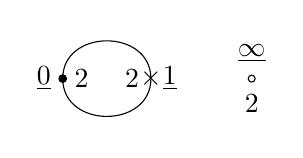
\begin{tikzpicture}[scale=.8]
\draw(0,0) .. controls (0,.8) and(1.4,.8)..(1.4,0) .. controls(1.4,-.8)and(0,-.8)..(0,0);
\fill(0,0)circle(.07);\node at(1.4,0){$\times$};\node at(-.3,0){$\underline0$};\node at(.3,0){$2$};\node at(1.1,0){$2$};\node at(1.7,0){$\underline1$};
\draw(3,0)circle(.055);\node at(3,.4){$\underline\infty$};\node at(3,-.4){$\unsure2$};\end{tikzpicture}}}
$G\xrightarrow{\sim}\unsure{\gamma_2}\xrightarrow{\sim}\mathbb Z_2=\deleted{\unsure{\mathbb Z_2}}\quad\unsure{\delta}=\unsure4$
\margin{$\begin{array}{ccc}&&1\\2&2&\deleted4\\&&1\end{array}$}
\deleted{$f(z)=z^2$}
\figure{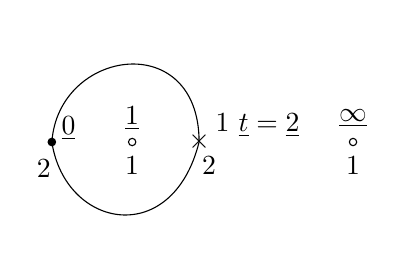
\begin{tikzpicture}[scale=.85]
\draw(0,0)..controls(.1,1.4)and(2.2,1.7)..(2.2,0)..controls(1.8,-1.6)and(.2,-1.3)..(0,0);
\fill(0,0)circle(.065);\node at(2.2,0){$\times$};\node at(.25,.2){$\underline0$};\node at(-.12,-.4){$2$};\node at(2.35,-.35){$2$};\node[right]at(2.3,.25){$\deleted1\ \underline t=\underline2$};
\draw(1.2,0)circle(.055);\node at(1.2,.35){$\underline1$};\node at(1.2,-.35){$1$};\draw(4.5,0)circle(.055);\node at(4.5,.35){$\underline\infty$};\node at(4.5,-.35){$1$};\end{tikzpicture}}
\[
\left[\begin{array}{l}
f(z)=\lambda\dfrac{z^2}{z-1}\\[4pt]
f(t)=\lambda\dfrac{t^2}{t-1}=1\\[4pt]
\left[f'(z)=\lambda\left(\dfrac{2z(z-1)-z^2}{(z-1)^2}\right)=\lambda\dfrac{z^2-2z}{(z-1)^2}=0\right]\\[4pt]
f'(t)=0\qquad t=2\qquad\lambda=\dfrac14
\end{array}\right]
\]
\[f(z)=\frac14\frac{z^2}{z-1}\]
$C^{\alpha}_{\mathcal C_0}$ a un seul él.

\textcircled{$\unsure{3'|3^a}$}
\figure{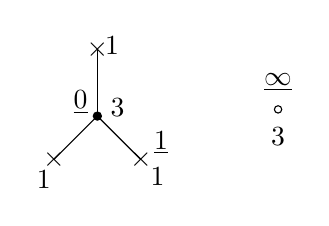
\begin{tikzpicture}[scale=.85]
\draw(0,0)--(0,1);\draw(0,0)--(-.65,-.65);\draw(0,0)--(.65,-.65);\fill(0,0)circle(.07);\node at(0,1){$\times$};\node at(-.65,-.65){$\times$};\node at(.65,-.65){$\times$};
\node at(.22,1.05){$1$};\node at(-.8,-.95){$1$};\node at(.9,-.9){$1$};\node at(.95,-.4){$\underline1$};\node at(-.25,.2){$\underline0$};\node at(.3,.12){$3$};\draw(2.7,.1)circle(.055);\node at(2.7,.5){$\underline\infty$};\node at(2.7,-.3){$3$};\end{tikzpicture}}
$G=\mathbb Z_3\subset\gamma\simeq\mathfrak S_3$
\margin{$\begin{array}{ccc}&1&\\3&1&3\\&1&\end{array}$}
\[f(z)=z^3\]
$C^{\alpha}_{\mathcal C_0}$ a deux éléments, $\gamma$ y est transitif, $\Gamma$ opère via le \unsure{caractère} cyclotomique des \unsure{racines $3$-èmes}.

\textcircled{$\unsure{3''|3^b}$}
\figure{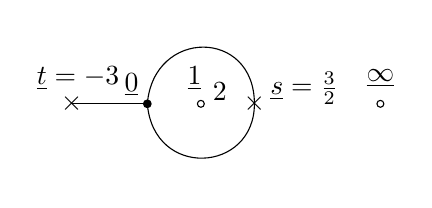
\begin{tikzpicture}[scale=.8]
\draw(-1.2,0)--(0,0);\draw(0,0)..controls(.1,1.2)and(1.7,1.2)..(1.7,0)..controls(1.7,-1.1)and(.1,-1.2)..(0,0);
\fill(0,0)circle(.07);\node at(-1.2,0){$\times$};\node at(1.7,0){$\times$};\node at(-1.1,.4){$\underline t=\unsure{-3}$};\node at(-.25,.3){$\underline0$};\node[right]at(1.8,.25){$\underline s=\frac32$};\draw(.85,0)circle(.055);\node at(.75,.4){$\unsure{\underline1}$};\node at(1.15,.2){$\deleted{\unsure2}$};\draw(3.7,0)circle(.055);\node at(3.7,.4){$\underline\infty$};\end{tikzpicture}}
$G\simeq\mathfrak S_3\qquad\gamma\simeq\{1\}$
\margin{$\begin{array}{ccc}&1&1\\3&2&2\end{array}$}
\[f(z)=\frac4{27}\frac{z^3}{z-1}\qquad\operatorname{Card}C^{\alpha}_{\mathcal C_0}=1\]

\scanpage{105}
% archive foliation: 104
\uline{NB} La figure barycentrique complète est la réunion de la droite $y(=\Im z)=0$, et de la courbe $2x(x^2+y^2)+(-3x^2+y^2)=0$
\figure{\begin{tikzpicture}[x=.8cm,y=.65cm]
\draw(-2.7,0)--(2.15,0);\draw(-2.05,5.1)..controls(-2.2,3.2)and(-1.4,1.5)..(0,0)..controls(.75,-1.3)and(2.1,-1.7)..(2.15,0)..controls(2.2,2.0)and(.8,1.8)..(0,0)..controls(-1.1,-1.7)and(-1.9,-3.5)..(-2,-5.2);
\draw[line width=1.15pt](0,0)..controls(.7,1.7)and(2.15,2)..(2.15,0)..controls(2.1,-1.6)and(.7,-1.4)..(0,0);
\fill(0,0)circle(.085);\node at(-2.7,0){$\times$};\node at(2.15,0){$\times$};\draw(1.4,0)circle(.085);
\foreach\x in {.15,.25,.35,.47,.59,.72,.84,.98,1.13,1.22,1.62,1.75,1.9}{\draw(\x,-.08)--(\x+.04,.08);}
\node at(-2.55,-.42){$-3$};\node at(0,-.4){$0$};\node at(1.46,-.35){$1$};\node[right]at(2.15,0){$\frac32$};
\end{tikzpicture}}

$\unsure{3''|3'''}$) (dual du précédent)
\figure{\begin{tikzpicture}[x=1cm,y=1cm]
\draw(0,0)--(2.2,0);\fill(0,0)circle(.06);\node at(.6,0){$\times$};\fill(1.15,0)circle(.06);\node at(2.2,0){$\times$};
\node at(0,-.35){$0$};\node at(.6,.4){$\frac13$};\node at(1.2,-.35){$1$};\node at(2.3,.4){$\frac43$};\draw(4.7,0)circle(.045);\node at(4.7,-.25){$\infty$};
\end{tikzpicture}}
\[f(z)=\frac{27}{4}z(z-1)^2\]
$\deleted{\unsure{\gamma\simeq}}G=\mathfrak S_3,\quad\gamma=\{1\}$
\[\operatorname{Card}C^{\alpha}_{\mathcal C_0}=1\]

\scanpage{106}
% archive foliation: 105
Montpellier \unsure{le|be} 11.1.1977

\deleted{Monsieur le Ministre,

Je me permets de recommander à votre attention le jeune mathéma-\newline
 ticien Kwang Taek Jeong, Chargé de Cours}

\figure{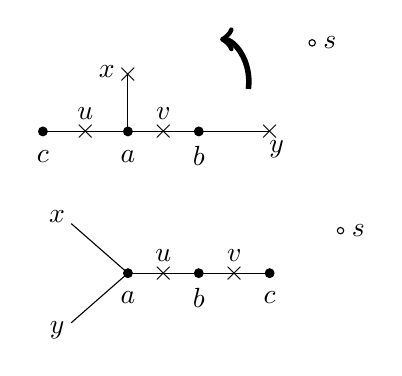
\begin{tikzpicture}[scale=.9]
\draw(-1.2,0)--(2,0);\draw(0,0)--(0,.8);\fill(-1.2,0)circle(.07);\fill(0,0)circle(.07);\fill(1,0)circle(.07);\node at(2,0){$\times$};\node at(0,.8){$\times$};\node at(-.6,0){$\times$};\node at(.5,0){$\times$};
\node at(-1.2,-.35){$c$};\node at(0,-.35){$a$};\node at(1,-.35){$b$};\node at(2.1,-.25){$y$};\node at(-.3,.85){$x$};\node at(-.6,.25){$u$};\node at(.5,.25){$v$};\draw(2.6,1.25)circle(.045);\node at(2.85,1.25){$s$};\draw[->,line width=2pt](1.7,.6)..controls(1.75,1)and(1.5,1.3)..(1.3,1.3);
\begin{scope}[yshift=-2cm]
\draw(-.8,.7)--(0,0)--(-.8,-.7);\draw(0,0)--(2,0);\fill(0,0)circle(.07);\fill(1,0)circle(.07);\fill(2,0)circle(.07);\node at(.5,0){$\times$};\node at(1.5,0){$\times$};\node at(-1,.8){$x$};\node at(-1,-.8){$y$};\node at(0,-.35){$a$};\node at(1,-.35){$b$};\node at(2,-.35){$c$};\node at(.5,.25){$u$};\node at(1.5,.25){$v$};\draw(3,.6)circle(.045);\node at(3.25,.6){$s$};\end{scope}
\end{tikzpicture}}
\diagram{$\begin{array}{ccc}3&2_2&\\2&1_2&6\\1&&\end{array}$}
\[\sigma_2\sigma_1\sigma_{\unsure1}\sigma_{\unsure2}=\]
\[\rho_s\rho_f=\sigma\qquad\rho_f=\rho_s^{-1}\sigma\]

\textcircled{I}
\diagram{$\begin{array}{llll}
r_1=(a,\unsure{ab})&\rho_s r_1=r_2&\sigma r_1=r_4&\rho_f r_1=r_5\\
r_2=(a,axa)&\rho_s r_2=r_3&\sigma r_4=r_1&\rho_f r_5=r_4\\
r_3=(a,ac)&\rho_s r_3=r_1&\sigma r_2=r_2&\rho_f r_4=r_3\\
r_4=(b,ba)&\rho_s r_4=r_5&\sigma r_3=r_6&\rho_f r_3=r_6\\
r_5=(b,byb)&\rho_s r_5=r_4&\sigma r_{\unsure6}=r_3&\rho_f r_6=r_2\\
r_6=(c,ca)&\rho_s r_6=r_6&\sigma r_5=r_5&\rho_f r_2=r_1
\end{array}$}
\figure{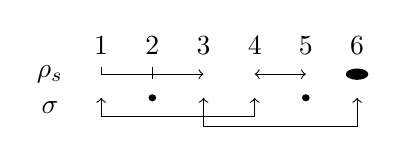
\begin{tikzpicture}[x=.65cm,y=.6cm]
\foreach\x in{1,...,6}{\node at(\x,1){$\x$};}
\node at(0,.4){$\rho_s$};\draw[->](1,.4)--(3,.4);\draw(1,.4)--(1,.55);\draw(2,.3)--(2,.55);\draw[<->](4,.4)--(5,.4);\fill(6,.4)ellipse(.22 and .12);
\node at(0,-.3){$\sigma$};\draw[<->](1,-.1)--(1,-.5)--(4,-.5)--(4,-.1);\draw[<->](3,-.1)--(3,-.7)--(6,-.7)--(6,-.1);\fill(2,-.1)circle(.075);\fill(5,-.1)circle(.075);
\end{tikzpicture}}
$\mathbb Z/6\mathbb Z$
\[p=6\quad q=2\quad r=6\]
\[N=\]

\textcircled{II}
\figure{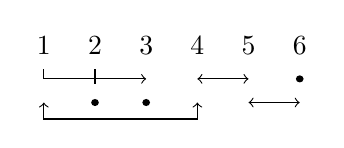
\begin{tikzpicture}[x=.65cm,y=.6cm]
\foreach\x in{1,...,6}{\node at(\x,1){$\x$};}
\draw[->](1,.3)--(3,.3);\draw(1,.3)--(1,.5);\draw(2,.2)--(2,.5);\draw[<->](4,.3)--(5,.3);\fill(6,.3)circle(.075);
\draw[<->](1,-.2)--(1,-.55)--(4,-.55)--(4,-.2);\fill(2,-.2)circle(.075);\fill(3,-.2)circle(.075);\draw[<->](5,-.2)--(6,-.2);
\end{tikzpicture}}
\diagram{$\begin{array}{llll}
r_1=(a,ab)&\rho_s r_1=r_2&\sigma r_1=r_4&\rho_f r_1=r_5\\
r_2=(a,axa)&\rho_s r_2=r_3&\sigma\unsure{\Delta}r_4=r_1&\rho_f r_5=r_6\\
r_3=(a,aya)&\rho_s r_3=r_1&\sigma r_2=r_2&\rho_f r_6=r_4\\
r_4=(b,ba)&\rho_s r_4=r_5&\sigma r_3=r_3&\rho_f r_4=r_3\\
r_5=(b,bc)&\rho_s r_5=r_{\unsure{4|2}}&\sigma r_5=r_6&\rho_f r_3=r_2\\
r_6=(c,cb)&\rho_s r_6=r_6&\sigma r_6=r_5&\rho_f r_2=r_1
\end{array}$}

\scanpage{107}
% archive foliation: 106
\deleted{
\[
\underline{\tau_{14}},\tau_{43}\text{ ou }\tau_{46}\ ?\qquad
\tau_{13}\text{ ou }\tau_{16}
\]
\[1\leq i\leq5\qquad\rho_s^i\sigma\rho_s^j\sigma\ldots\rho_s^h\sigma\]
\[\rho_s^{\unsure3}=(\tau_{4,5})\qquad\rho_s^4=(1,2,3)(4)(5)(6)\]
}
\deleted{$(fgh)'=(fg)'h+(fg)h'=\unsure{f'gh|fg'h}+fg'h+fgh'$}

\[a=\underline0\quad\underline b=1\qquad\unsure{s}=\underline\infty\]
\uline{reste}\quad$c,x,y,u,v$
\[f(z)=\lambda\uuline{z^3(z-1)^2(z-c)}\]
\[
\left\{\begin{array}{ll}\underline0&\text{zéro triple}\\\underline1&\text{zéro double}\\c&\text{zéro simple}\end{array}\right.
\qquad\left\{\infty\text{ pôle d'ordre }6\right.
\]
\[
\begin{aligned}
f'(z)&=\lambda\deleted{\unsure{f}}\bigl[z^2(z-1)(\underbrace{3(z-1)(z-c)+2z(z-c)}_{(5z-3)(z-c)}+z(z-1))\bigr]\\
&=\lambda z^2(z-1)[6z^2-(5c+4)z+3c]
\end{aligned}
\]
Ses zéros distincts de $0,1,\infty$ sont les zéros de
\[6z^2-(5c+4)z+3c=0\]
\deleted{\unsure{soient}} $u,v$. Il faut donc \deleted{\unsure{écrire} $f$}
\deleted{\illegible{1}\unsure{que}}
\[
\left\{\begin{array}{l}u,v\text{ distincts entre eux et }\ne0,1,c\\f(u)=f(v)=1\end{array}\right.
\qquad\text{(racines doubles de cette équation}
\]
\[f(z)-1=\deleted{\unsure{\lambda z^2}}\ \lambda(z-u)^2(z-v)^2(z-x)(z-y)\]

\scanpage{108}
% archive foliation: 107
\[
u^2=\alpha u+\beta\qquad\alpha=\frac{5c}{6}+\frac23,\quad\beta=-\frac c2
\]
\[
\frac1\lambda f(u)=\deleted{\unsure z}\underbrace{u(\alpha u+\beta)}_{\substack{\deleted{\unsure{\beta u}}\\(\alpha^2+\beta)u+\alpha\beta}}
\underbrace{((\alpha-2)u+(\beta+1))(u-c)}_{\substack{\underbrace{(\alpha-2)u^2+[(\beta+1)-c(\alpha-2)]u-(\beta+1)c}}}
\]
\[
(\underbrace{(\alpha-2)\alpha+\beta+1-c(\alpha-2)}_{(\alpha-2)(\alpha-c)+(\beta+1)})u+((\alpha-2)\beta-(\beta+1)c)
\]
\[
\begin{aligned}
&\alpha(\alpha^2+\beta)[(\alpha-2)\unsure{(\alpha-c)|\alpha}+\beta+1]\deleted{\unsure{u+c(\alpha-2)}}
+\beta(\alpha^2+\beta)[(\alpha-2)(\alpha-c)+\beta+1]\\
&+\alpha\beta[(\alpha-2)(\alpha-c)+\beta+1]u
\qquad+\alpha\beta[(\alpha-2)\beta-(\beta+1)c]\\
&+(\alpha^2+\beta)[(\alpha-2)\beta\unsure{+|-}(\beta+1)c]u
\end{aligned}
\]
\deleted{$[(\alpha-2)(\alpha-c)+\beta+1][(\alpha^2+\beta)(\alpha+1)+\alpha\beta]$}
\[
\begin{aligned}
\alpha-2&=\frac{5c}{6}-\frac43\\
\alpha-c&=-\frac c6+\frac23\\
(\alpha-2)(\alpha-c)&=-\frac5{36}c^2+\frac79c-\frac89\\
\beta+1&=-\frac c2+1=-\frac{\unsure9c}{18}+\frac99
\end{aligned}
\]
\[
(\alpha-2)(\alpha-c)+\beta+1=-\frac5{36}c^2+\frac5{18}c+\frac19
=-\frac1{36}(\deleted{\unsure5}5c^2\unsure{-|+}10c-4)
\]
\[
\begin{aligned}
\alpha^3+2\alpha\beta
&=\deleted{\frac{(5c+4)^3}{6^3}\unsure{-|+}\frac{c(5c+4)}6=\frac1{6^3}\underbrace{[(5c+4)^2-36c(5c+4)]}_{\substack{\deleted{-165c^2-}\\(5c+4)(-29c+4)}}}\\
&=\alpha(\alpha^2+2\beta)=\frac1{6^3}(5c+4)((5c+4)^2-36c)\\
&=\frac1{6^3}(5c+4)(25c^2+4c+16)
\end{aligned}
\]
\[ -\frac16\left(\frac56\right)^4c^5 \]

\scanpage{109}
% archive foliation: 108
\[
\begin{aligned}
\lambda(P(c)u+Q(c))&=1\\
\lambda(P(c)v+Q(c))&=1
\end{aligned}
\]
\[P(c)(u-v)=0\]
\[\boxed{P(c)=0}\qquad\lambda=\frac1{Q(c)}\]
\[Q(c)\ne0\]
\figure{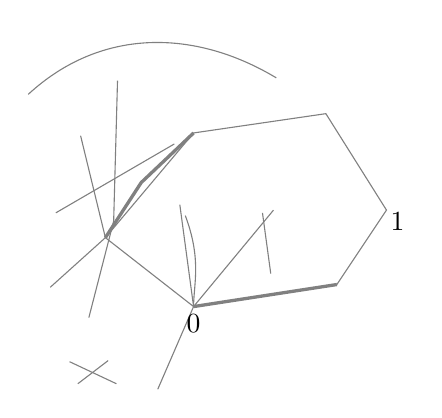
\begin{tikzpicture}[scale=.7]
\draw[gray](-2,2.8)..controls(-.7,4)and(1,4)..(2.5,3.1);
\draw[gray](-.6,.2)--(1,2.1)--(3.4,2.45)--(4.5,.7)--(3.6,-.65)--(1,-1.05)--cycle;
\draw[gray,line width=1.2pt](-.6,.2)--(.05,1.2)--(1,2.1);\draw[gray,line width=1.2pt](1,-1.05)--(3.6,-.65);
\draw[gray](-1.6,-.7)--(-.6,.2)--(-1.05,2.05);\draw[gray](-.9,-1.25)--(-.45,.5)--(-.38,3.05);\draw[gray](-1.5,.65)--(.65,1.9);
\draw[gray](.35,-2.55)--(1,-1.05)--(.75,.8);\draw[gray](.85,.6)..controls(1.15,-.2)and(1,-.65)..(1,-1.05);\draw[gray](1,-1.05)--(2.45,.7);\draw[gray](2.4,-.45)--(2.25,.65);
\draw[gray](-1.25,-2.05)--(-.4,-2.45);\draw[gray](-1.1,-2.45)--(-.55,-2.03);
\node at(1,-1.35){$0$};\node at(4.7,.5){$1$};\end{tikzpicture}}
\margin{$\unsure{\widetilde X}\quad\underline a$}

\[\unsure{\mathcal P}\qquad
\boxed{\begin{array}{l}c\ne0,1\\Q(c)\ne0\\P(c)=0\end{array}}\qquad
f(z)=\frac1{Q(c)}z^3(z-1)^2(z-c)
\]
\[\boxed{(5c+4)^2-72c\ne0}\]
\figure{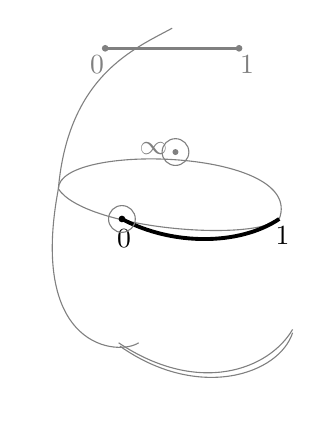
\begin{tikzpicture}[scale=.85]
\draw[gray,line width=1.2pt](0,2.5)--(2,2.5);\fill[gray](0,2.5)circle(.05);\fill[gray](2,2.5)circle(.05);\node[gray]at(-.12,2.25){$0$};\node[gray]at(2.12,2.25){$1$};
\draw[gray](-.7,.4)..controls(-.55,2.1)and(.45,2.5)..(1,2.8);\draw[gray](-.7,.4)..controls(-1.15,-2)and(.2,-2.1)..(.5,-1.9);\draw[gray](-.7,.4)..controls(-.3,-.2)and(2.2,-.4)..(2.6,-.05)..controls(3,1)and(-.7,1.1)..(-.7,.4);
\draw[gray](.2,-1.9)..controls(1.4,-2.7)and(2.45,-2.3)..(2.8,-1.7);\draw[gray](.22,-1.95)..controls(1.4,-2.78)and(2.6,-2.37)..(2.8,-1.75);
\draw[line width=1.4pt](.25,-.05)..controls(1,-.45)and(2,-.45)..(2.6,-.05);\fill(.25,-.05)circle(.05);\node at(.28,-.35){$0$};\node at(2.65,-.3){$1$};\draw[gray](.25,-.05)circle(.2);
\fill[gray](1.05,.95)circle(.045);\draw[gray](1.05,.95)circle(.2);\node[gray]at(.72,1){$\infty$};\end{tikzpicture}}
\figure{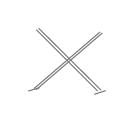
\begin{tikzpicture}[scale=.6]\draw[gray](-.7,-.6)--(.7,.6);\draw[gray](-.65,-.62)--(.75,.58);\draw[gray](-.65,.65)--(.65,-.65);\draw[gray](-.6,.68)--(.72,-.63);\draw[gray](-.82,-.65)--(-.58,-.58);\draw[gray](.58,-.72)--(.82,-.64);\end{tikzpicture}}

$u,v$ sont les racines de
\[\deleted{\unsure{f(z)}}\ z^2-\frac{5c+4}{6}z+\frac c2=0\]
$x,y$ sont les racines de
\figure{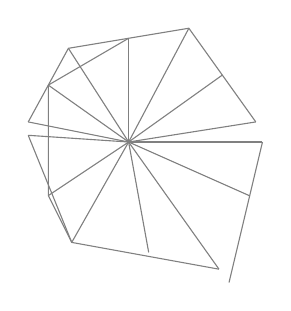
\begin{tikzpicture}[scale=.85]
\coordinate(O)at(0,0);\draw[gray](-1.5,.3)--(-.9,1.4)--(.9,1.7)--(1.9,.3);\draw[gray](-1.5,.1)--(-.85,-1.5)--(1.35,-1.9);\draw[gray](2,0)--(1.5,-2.1);
\foreach\p in{(-1.5,.3),(-1.2,.85),(-.9,1.4),(0,1.55),(.9,1.7),(1.4,1),(1.9,.3),(2,0),(1.8,-.8),(1.35,-1.9),(.3,-1.65),(-.85,-1.5),(-1.2,-.8),(-1.5,.1)}{\draw[gray](O)--\p;}
\draw[gray](-1.2,.85)--(-1.2,-.8)--(-.85,-1.5);\draw[gray](-1.2,.85)--(0,1.55);\end{tikzpicture}}
\[
\frac{f(z)-1}{(z-u)^2(z-v)^2}=\frac{f(z)\unsure{+|-}1}{\left(z^2-\frac{5c+4}{6}z+\frac c2\right)^2}
\]

\scanpage{110}
% archive foliation: 109
\begin{center}
U N I V E R S I T E\\
DES SCIENCES ET TECHNIQUES\\
DU LANGUEDOC\\
------------\\
Service de la Scolarité\\
JP/GJ\\
Diffusion : Liste H\\
N°7119
\end{center}
Montpellier, le 12 Décembre 1977

\uline{AVIS DE SOUTENANCE D'UNE THESE DE DOCTORAT D'ETAT}

\uline{Nom et prénom du candidat} : COMBE Michel, Gaston, Fernand

\uline{Titre de la thèse} : Ressources en Eau du Maroc avec application à la méthodologie de la représentation des systèmes aquifères et de leur fonctionnement.

\uline{Date, heure et lieu de soutenance prévus} : 21 DECEMBRE 1977 à 15h30 mn\\
Salle de cours n° 6 - U.S.T.L.

\uline{Nom du directeur de thèse} : Monsieur le Professeur J. AVIAS

\uline{Désignation du laboratoire où la thèse est préparée} : CERGH (Pr AVIAS)

\uline{Résumé de la thèse} : Trois volumes publiés dans la série des Notes et Mémoires du Service Géologique du Maroc n° 231 ont été rédigés sous la direction du candidat entre 1967 et 1977 avec la participation d'hydrogéologues régionaux (1200 pages - 508 figures). Ils synthétisent pour les 46 bassins hydrogéologiques du Maroc les données climatologiques, géologiques, hydrologiques, hydrogéologiques et présentent un bilan des ressources en eau et des utilisations ainsi que des orientations pour la poursuite des recherches. Un quatrième volume synthétise l'ensemble sous forme d'une carte au 1/1.000.000 des systèmes aquifères et de leur fonctionnement qui est une cartographie hydrogéologique \unsure{nouvelle}, totalement affranchie des représentations géologiques habituelles.

\uline{Durée approximative des recherches ayant abouti à la thèse} : 15 ans

\uline{Nom des rapporteurs} :\\
M. AVIAS J., Professeur,Hydrogéol.,U.S.T.L.\\
M. MARGAT J., Conseiller scientifique, BRGM\\
M. CASTANY G.,Conseiller scientifique, BRGM

\figure{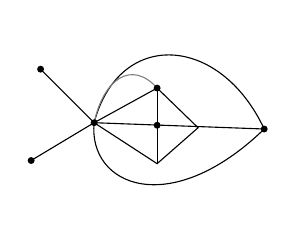
\begin{tikzpicture}[scale=.8]
\draw(-.85,.85)--(0,0)--(-1,-.6);\draw(0,0)..controls(.4,1.5)and(2,1.4)..(2.7,-.1)..controls(1.2,-1.55)and(-.1,-1)..(0,0);
\draw(0,0)--(1,.55)--(1.65,-.08)--(1,-.65)--cycle;\draw(1,.55)--(1,-.65);\draw(0,0)--(2.7,-.1);\draw[gray](0,0)..controls(.15,.7)and(.6,1)..(1,.55);
\foreach\p in{(-.85,.85),(-1,-.6),(0,0),(1,.55),(1,-.04),(2.7,-.1)}{\fill\p circle(.055);}
\end{tikzpicture}}

\uline{Composition du jury} :\\
M. AVIAS J., Professeur, Hydrogéologie, U.S.T.L. (Président)\\
M. BOCQUILLON Cl., Professeur, \unsure{Hydrogéologie}, U.S.T.L.\\
M. CASTANY G., Conseiller scientifique, B.R.G.M.\\
M. MARGAT J., Conseiller scientifique, B.R.G.M.\\
(Membre extérieur choisi en raison de sa compétence scientifique)\\
M. AMBROGGI R., Expert international FAO ROME\\
M. LOUIS\qquad Professeur, Géophysique, U.S.T.L.\\
(Membre étranger à la spécialité du candidat).

\margin{$=6N$\\$2(\sum p+\sum q+\sum r)$}

Le Secrétaire Général,

\unsure{E. Siau}

\uline{E. SIAU}

\figure{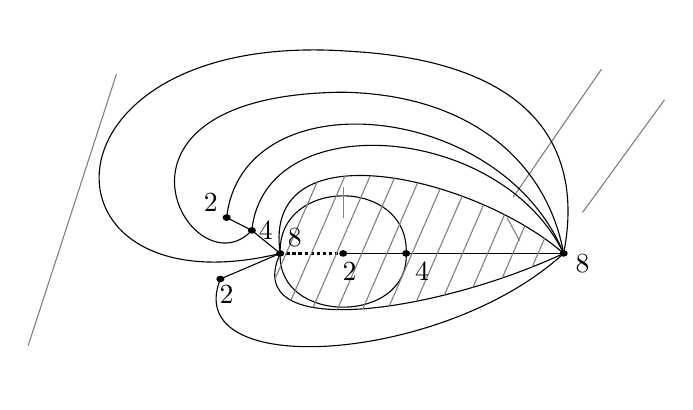
\begin{tikzpicture}[x=.8cm,y=.65cm]
\coordinate(A)at(0,0);\coordinate(B)at(4.5,0);
\draw[gray](-4,-1.8)--(-2.6,3.5);\draw[gray](5.1,3.6)--(3.7,1.1);\draw[gray](6.1,3)--(4.8,.8);
\draw(A)--(-.45,.45)--(-.85,.7);\draw(A)--(-.95,-.5);\draw[densely dotted,line width=1.2pt](A)--(1,0);\draw(1,0)--(B);
\draw(A)..controls(-.05,1.5)and(2.05,1.5)..(2,0)..controls(2.05,-1.4)and(-.05,-1.4)..(A);
\draw(A)..controls(-.3,2.5)and(3.1,1.5)..(B);
\draw(A)..controls(-.65,-1.75)and(2.5,-1.15)..(B);
\draw(-.45,.45)..controls(-.25,2.9)and(3.5,2.55)..(B);
\draw(-.85,.7)..controls(-.6,3.45)and(3.5,3)..(B);
\draw(-.45,.45)..controls(-1.4,-.8)and(-3.25,3.1)..(1,3.15)..controls(3.1,3.1)and(4.25,1.7)..(B);
\draw(A)..controls(-4,-1.2)and(-4,4.4)..(1.1,3.95)..controls(4.7,3.7)and(4.7,1.25)..(B);
\draw(-.95,-.5)..controls(-1.6,-2.5)and(2.6,-2.15)..(B);
\begin{scope}\clip(A)..controls(-.3,2.5)and(3.1,1.5)..(B)..controls(2.5,-1.15)and(-.65,-1.75)..(A);\foreach\x in{-.4,0,.4,...,4.4}{\draw[gray](\x,-1.4)--(\x+1.2,2);}\end{scope}
\foreach\p in{(0,0),(4.5,0),(-.45,.45),(-.85,.7),(-.95,-.5),(1,0),(2,0)}{\fill\p circle(.065);}
\node at(-1.1,1){$2$};\node at(-.23,.45){$4$};\node at(.23,.3){$8$};\node at(-.85,-.8){$2$};\node at(1.1,-.35){$2$};\node at(2.25,-.35){$4$};\node at(4.8,-.2){$8$};\draw[gray](1,1.3)--(1,.7);\draw[gray](3.6,.7)--(3.8,.25);
\end{tikzpicture}}
\figure{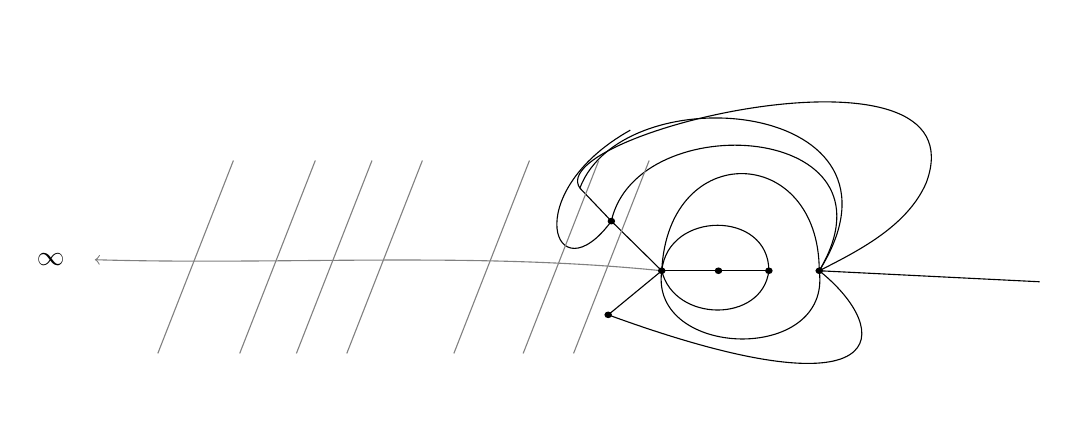
\begin{tikzpicture}[x=.8cm,y=.7cm]
\coordinate(A)at(0,0);\coordinate(B)at(2.5,0);
\draw[gray,->](A)..controls(-3,.35)and(-6,.1)..(-9,.2);\node at(-9.7,.2){$\infty$};\draw(B)--(6,-.2);
\draw(A)--(-.8,.9)--(-1.3,1.5);\draw(A)--(-.85,-.8);\draw(A)--(1.7,0);
\draw(A)..controls(.1,1.1)and(1.7,1.1)..(1.7,0)..controls(1.6,-.95)and(.2,-.95)..(A);
\draw(A)..controls(.1,2.4)and(2.5,2.3)..(B)..controls(2.7,-1.7)and(-.2,-1.6)..(A);
\draw(-.8,.9)..controls(-.4,3)and(3.9,2.7)..(B);
\draw(-1.3,1.5)..controls(-.6,3.6)and(4.2,3.1)..(B);
\draw(-1.3,1.5)..controls(-1.9,2.5)and(5.1,4.4)..(4.2,1.6)..controls(3.9,.8)and(3.1,.35)..(B);
\draw(-.8,.9)..controls(-1.7,-.5)and(-2.3,1.4)..(-.5,2.55);
\draw(-.85,-.8)..controls(3.7,-2.7)and(3.7,-1.1)..(B);
\foreach\p in{(0,0),(2.5,0),(-.8,.9),(-.85,-.8),(.9,0),(1.7,0)}{\fill\p circle(.06);}
\foreach\x in{-8,-6.7,-5.8,-5,-3.3,-2.2,-1.4}{\draw[gray](\x,-1.5)--(\x+1.2,2.0);}
\end{tikzpicture}}

\scanpage{111}
% archive foliation: 110
\[
f(z)-1=\lambda z^3(z-1)^2(z-c)-1\quad\text{divisible par}\quad
(z^2-\alpha z\unsure{-}\beta)^2
\]
\[
\lambda z^3(z-1)^2(z-c)\inserted{-1}=\lambda(z^2-\alpha z-\beta)^2(z^2+lz+m)
\]
\figure{\begin{tikzpicture}\draw (0,0)--(2,0);\end{tikzpicture}}
\[
c=0\qquad z^2-\frac23z=0\qquad\text{solutions}\quad
\begin{array}{l}u=0\\v=\frac23\end{array}
\]
\[
\frac1\lambda f=\begin{array}{l}\deleted{z^4(z-1)^2}\\z^3(z-1)^3\end{array}
\qquad \deleted{f=\lambda z^4(z-1)^{\unsure{2}}}
\]
\[
\deleted{\unsure{6}}z^2-\frac32z+\frac12=0
\qquad(z-1)(z\unsure{-}\tfrac12)
\]
\[
\begin{array}{l}
u\deleted{P(c)}+\deleted{\unsure{u}}Q(c)=0\\
v\deleted{P(c)}+\deleted{\unsure{v}}Q(c)\ne0\\[3pt]
P(c)=0
\end{array}
\qquad P(c)=0\Rightarrow c\ne0,1
\]
\[
\underbrace{25c^2-32c+16}_{\delta(c)}
\qquad\begin{array}{l}32^{\unsure2}(32-50)\\-32.18\\=-(8.3)^2\\[3pt]
c=\dfrac{16}{25}\pm\dfrac{24}{25}i\end{array}
\]
\[
\mathbb Q[c]_{\delta(c)c(c-1)}/P(c)Q(c)
\]
\[
\mathbb Q[c]_{\delta(c)Q(c)}
\qquad P(c)=Q(c)=0\quad\Rightarrow\quad f(u)=f(v)=0
\]
\margin{$u,v$ sont parmi les valeurs $0,1,c$.}
\[
\begin{array}{ll}
a)\ u=0&\Rightarrow c=0\quad\text{absurde}\\
b)\ u=1&\Rightarrow 6-(5c+4)+3c=0\\
&\text{i.e. }2-2c=0\quad\text{i.e. }c=1\quad\text{absurde}\\
c)\ u=c&6c^2-(5c+4)c+3c=0\\
&c^2-c=0\quad c(1-c)=0\quad c=0\ \text{ou}\ c=1\quad\text{absurde}
\end{array}
\]

\scanpage{112}
% archive foliation: 111
Donc on voit que les zéros de $P(c)$ sont distincts de $0,1$ et ne sont pas des zéros de $Q$. Mais pourraient-ils être zéros de
\[
\delta(c)=25c^2-32c+16\quad ?
\]
\figure{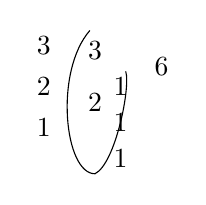
\begin{tikzpicture}[scale=.65]
\node at (0,2){$3$};\node at (0,1.2){$2$};\node at (0,.4){$1$};
\node at (1,1.9){$3$};\node at (1,.9){$\deleted{\unsure{2}}$};
\node at (1.5,1.2){$1$};\node at (1.5,.5){$1$};\node at (1.5,-.2){$1$};
\draw (.9,2.3)..controls(.2,1.5)and(.4,-.5)..(1,-.5)..controls(1.4,-.3)and(1.7,1.2)..(1.6,1.5);
\node at (2.3,1.6){$6$};\end{tikzpicture}}
\[
f'(z)=0\Rightarrow f(z)=0
\]
\deleted{\figure{\begin{tikzpicture}[scale=.6]
\node at(-.8,1){\unsure{ou}};\node at(0,1){$3$};\node at(0,.4){$2$};\node at(0,-.3){$1$};\draw(0,.35)ellipse(.4 and1);
\node at(1.4,.7){$\unsure{0}$};\node at(3.4,1){$3$};\node at(3.4,.1){$1_3$};\draw(3.4,.5)ellipse(.25 and.9);
\draw(-.7,.7)..controls(1,1.8)and(.4,-.5)..(1.5,.6)..controls(2.4,1)and(1.5,-.1)..(3.8,.8);
\end{tikzpicture}}}
\[
f(z)=\lambda\frac{\varphi}{\psi}
\]
\margin{$\varphi,\psi$ \inserted{unitaires} premiers entre eux à zéros indéterminés de multiplicités données, $\deg\varphi>\deg\psi$}
\[
\frac{f'(z)}{\inserted{f(z)}}=
\deleted{\frac\lambda{\psi^2}}
\left(\frac{\varphi'}{\inserted{\varphi}}\deleted{\psi}
-\frac{\psi'}{\inserted{\psi}}\deleted{\varphi}\right)
\]
\[
\sum\frac{p_i}{z-\alpha_i}\ \unsure{*}\ \unsure{-}\sum\frac{\unsure{5|q_j}}{\unsure{z}-\beta_j}
\]
\[
=\frac1{\prod(z-\alpha_i)\prod(z-\beta_j)}\;\bigl(\qquad\bigr)
\]

\scanpage{113}
% archive foliation: 112
\margin{Cartes sphériques en bas degrés}

\scanpage{114}
% archive foliation: 113
\figure{\begin{tikzpicture}[scale=.7,line cap=round,line join=round]
\begin{scope}[shift={(1,8)}]
\draw (0,0)..controls(-1,1)and(1.3,2.5)..(2,1.8)..controls(2.7,1.2)and(1.2,-.2)..(0,0);
\draw[very thick](0,0)--(1.4,.2)--(1.2,1.2)--(2,1.8);\draw(1.2,1.2)..controls(1.8,1.2)..(2,1.8);
\foreach \p in {(0,0),(1.4,.2),(1.2,1.2),(2,1.8)}\fill\p circle(2pt);\end{scope}
\begin{scope}[shift={(5,8)}]
\draw(0,-.2)..controls(-.4,1)and(1,1.7)..(2,1.7)..controls(2.8,1.3)and(2.2,-1)..(1.5,-.4)..controls(.6,-.8)..(0,-.2);
\draw(2,1.7)--(1.25,.85)--(1.5,-.4);
\foreach \p in {(0,-.2),(2,1.7),(1.65,1.3),(1.25,.85),(1.5,-.4)}\fill\p circle(2pt);
\node at(.7,.7){$5$};\node at(1.9,.65){$4$};\end{scope}\node at(9,8.7){$3$};
\draw(-.8,5.2)..controls(-.8,6.1)and(.4,6.4)..(.4,5.8);
\begin{scope}[shift={(3,5.6)}]
\draw[thick](0,0)..controls(-.6,1.2)and(1.7,1.8)..(1.5,.35)..controls(1,-.7)..(0,0);
\draw(0,0)..controls(1.5,.2)and(.8,1.1)..(0,0);\draw(1.5,.35)--(2.3,.3);
\foreach\p in{(0,0),(.35,1.05),(1.5,.35)}\fill\p circle(2pt);
\node at(.55,.35){$1$};\node at(1, .9){$3$};\node at(1.9,-.15){$\unsure{4|5}$};
\draw(-.6,1.5)..controls(-1.8,-2)and(4,-2)..(2.5,.9)..controls(1.7,2.4)..(-.6,1.5);\node at(1.4,-1.2){$8$};\end{scope}
\begin{scope}[shift={(.5,3.7)}]
\draw(0,0)..controls(-.6,.9)and(.2,2)..(1,1.3)..controls(2,.3)and(1,-.8)..(0,0);
\draw(-.6,-.6)--(0,0)--(.9,.9);\draw(1.5,.55)--(2.3,.55);
\foreach\p in{(0,0),(-.05,.7),(.55,1.4),(1.5,.55)}\fill\p circle(2pt);
\draw(.2,.25)--(.4,.6)--(.6,.6)--(.7,.8)--(.9,.9)--(.85,.65);
\node at(.8,.3){$3$};\node at(2,.05){$\unsure{5|4}$};\end{scope}
\begin{scope}[shift={(6.3,6.2)}]
\draw[very thick](-.7,0)--(2.1,0);\draw(0,0)--(0,1.2);
\foreach\p in{(0,0),(0,.65),(0,1.2),(.65,0),(1.3,0),(2,0)}\fill\p circle(2pt);
\draw(-.7,-.2)--(-.95,-.25)--(-.7,-.3);\draw(1.9,0)--(2.1,.13)--(2.25,-.07);
\end{scope}
\begin{scope}[shift={(6.3,4.3)}]
\draw(-.7,0)--(1.7,0);\draw(0,0)--(0,1.1);
\foreach\p in{(0,0),(0,.6),(.5,0),(1.05,0)}\fill\p circle(2pt);
\draw(-1,1.1)..controls(-2,-1.5)and(.2,-2.4)..(2.7,-1.1)..controls(4,1.8)and(-.1,2.2)..(-1,1.1);
\node at(.5,-.7){$\deleted{\unsure{9}}$};\node at(1.6,-1.9){$9$};\end{scope}
\begin{scope}[shift={(10.3,6.8)}]
\draw(-.7,0)--(1.2,0);\draw(0,-.5)--(0,.55);\foreach\p in{(-.7,0),(0,0),(.65,0),(1.2,0)}\fill\p circle(1.5pt);\draw(0,.5)--(.1,.65)--(-.05,.6);
\end{scope}
\begin{scope}[shift={(10.3,5)}]\draw(-.45,.3)--(.35,-.25);\draw(-.35,-.4)--(0,0)--(0,.5);\end{scope}
\begin{scope}[shift={(10.3,1.8)}]
\draw[thick](-.9,0)--(.7,0);\draw(0,0)--(0,.5);\foreach\p in{(-.5,0),(0,0),(.7,0)}\fill\p circle(2pt);
\draw(0,-.3)ellipse(1.7 and1);\node at(0,-.7){$6$};\node at(0,.95){$\deleted{\unsure{4}}$};\end{scope}
\draw(6.5,0)--(7.1,0);\fill(7.1,0)circle(1.5pt);
\end{tikzpicture}}
\figure{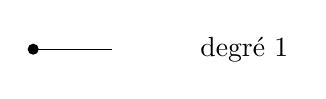
\begin{tikzpicture}\fill(0,0)circle(2pt);\draw(0,0)--(1,0);\node[right]at(2,0){degré $1$};\end{tikzpicture}}
\deleted{\figure{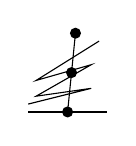
\begin{tikzpicture}\draw(0,0)--(1,0);\draw(.5,0)--(.6,1);\foreach\p in{(.5,0),(.55,.5),(.6,1)}\fill\p circle(2pt);\draw(0,.1)--(.8,.3)--(.1,.2)--(.8,.6)--(.1,.4)--(.9,.9);\end{tikzpicture}}}
\[
n=\sum_s q_s=\sum_f p_f
\]
\uline{degré $1$}\qquad $\unsure{\varphi(1)|\varphi(n)}=2$
\figure{\begin{tikzpicture}\fill(0,0)circle(2pt);\draw(.15,0)--(1,0);\end{tikzpicture}}
\uline{degré $2$}\quad a) $1$ seul sommet d'ordre $2$
\figure{\begin{tikzpicture}\draw(-1,0)--(1,0);\fill(0,0)circle(2pt);\node at(0,.45){\deleted{\unsure{2 arêtes}}};
\begin{scope}[shift={(3,0)}]\draw(0,0)..controls(-1,1.5)and(1.5,1.5)..(0,0);\fill(0,0)circle(2pt);\end{scope}
\draw(4.5,.2)--(5.2,.1)--(4.5,.25)--(5.3,.05);\end{tikzpicture}}
b) $2$ sommets d'ordre $1$
\figure{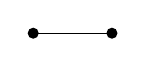
\begin{tikzpicture}\draw(0,0)--(1,0);\fill(0,0)circle(2pt);\fill(1,0)circle(2pt);\end{tikzpicture}}
\uline{degré $3$}\quad a) $1$ sommet d'ordre $3$
\figure{\begin{tikzpicture}\draw(-1,0)--(0,0)--(.5,.6);\draw(0,0)--(.4,-.6);\fill(0,0)circle(2pt);
\draw(2,-.2)--(2.6,.1)..controls(2.6,1.6)and(4.1,.3)..(2.6,.1);\fill(2.6,.1)circle(2pt);\end{tikzpicture}}
b) $2$ sommets, d'ordre $1$ et $2$
\deleted{\figure{\begin{tikzpicture}\draw(0,0)ellipse(.6 and.35);\draw(-.5,.3)--(.3,.25)--(-.4,.1)--(.6,.1)--(-.4,-.15)--(.2,-.25);\end{tikzpicture}}}
\figure{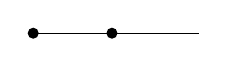
\begin{tikzpicture}\draw(1.3,0)--(3.4,0);\fill(1.3,0)circle(2pt);\fill(2.3,0)circle(2pt);\end{tikzpicture}}
\uline{degré $4$}\quad a) $1$ sommet d'ordre $4$
\figure{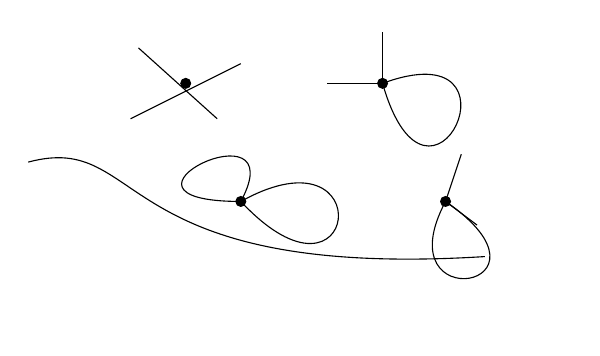
\begin{tikzpicture}
\draw(-.7,-.45)--(.7,.25);\draw(-.6,.45)--(.4,-.45);\fill(0,0)circle(2pt);
\begin{scope}[shift={(2.5,0)}]\draw(-.7,0)--(0,0)--(0,.65);\draw(0,0)..controls(1.9,.7)and(.6,-2.1)..(0,0);\fill(0,0)circle(2pt);\end{scope}
\begin{scope}[shift={(.7,-1.5)}]\draw(0,0)..controls(-2,0)and(.7,1.3)..(0,0)..controls(1.8,1)and(1.5,-1.6)..(0,0);\fill(0,0)circle(2pt);\end{scope}
\begin{scope}[shift={(3.5,-1.5)}]\draw(0,.6)--(-.2,0)--(.2,-.3);\draw(-.2,0)..controls(-1,-1.5)and(1.4,-1.1)..(-.2,0);\fill(-.2,0)circle(2pt);\end{scope}
\draw(-2,-1)..controls(-.5,-.6)and(-1,-2.5)..(3.8,-2.2);
\end{tikzpicture}}
b) $1$ sommet d'ordre $3$, $1$ d'ordre $1$
\figure{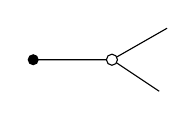
\begin{tikzpicture}\draw(0,0)--(1,0)--(1.7,.4);\draw(1,0)--(1.6,-.4);\fill(0,0)circle(2pt);\draw[fill=white](1,0)circle(2pt);\end{tikzpicture}}
\deleted{\figure{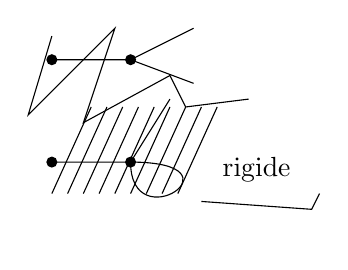
\begin{tikzpicture}
\draw(0,0)--(1,0)--(1.8,.4);\draw(1,0)--(1.8,-.3);\fill(0,0)circle(2pt);\fill(1,0)circle(2pt);
\draw(0,-1.3)--(1,-1.3)--(1.5,-.5);\draw(1,-1.3)..controls(2.5,-1.3)and(1,-2.3)..(1,-1.3);\fill(0,-1.3)circle(2pt);\fill(1,-1.3)circle(2pt);
\foreach\x in{0,.2,...,1.7}\draw(\x,-1.7)--(\x+.5,-.6);
\draw(0,.3)--(-.3,-.7)--(.8,.4)--(.4,-.8)--(1.5,-.2)--(1.7,-.6)--(2.5,-.5);
\node at(2.6,-1.4){\unsure{rigide}};\draw(1.9,-1.8)--(3.3,-1.9)--(3.4,-1.7);
\end{tikzpicture}}}

\scanpage{115}
% archive foliation: 114
\figure{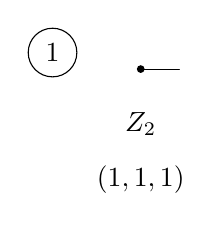
\begin{tikzpicture}[scale=.7,line cap=round]
\node[draw,circle]at(-1.6,.3){$1$};
\begin{scope}[shift={(0.0,0)}]\draw(0,0)--(.7,0);\fill(0,0)circle(2pt);
\node at(0,-1.0){$\uuline{\mathbb Z_2}$};
\node at(0,-2.0){$\left(1,1,1\right)$};
\end{scope}
\end{tikzpicture}}
\figure{\begin{tikzpicture}[scale=.7,line cap=round]
\node[draw,circle]at(-1.6,.3){$2$};
\begin{scope}[shift={(0.0,0)}]\draw(-.7,0)--(.7,0);\fill(0,0)circle(2pt);
\node at(0,-1.0){$\uuline{\mathbb Z_2\times\mathbb Z_2}$};
\node at(0,-2.0){$\left(2,\begin{smallmatrix}1\\1\end{smallmatrix},2\right)$};
\end{scope}
\begin{scope}[shift={(3.1,0)}]\draw(-.5,0)--(.5,0);\fill(-.5,0)circle(2pt);\fill(.5,0)circle(2pt);
\node at(0,-1.0){$\uuline{\mathbb Z_2\times\mathbb Z_2}$};
\node at(0,-2.0){$\left(\begin{smallmatrix}1\\1\end{smallmatrix},2,2\right)$};
\end{scope}
\begin{scope}[shift={(6.2,0)}]\fill(0,0)circle(2pt);\draw(0,0)..controls(1.3,1.4)and(1.4,-1)..(0,0);
\node at(0,-1.0){$\uuline{\mathbb Z_2\times\mathbb Z_2}$};
\node at(0,-2.0){$\left(2,2,\begin{smallmatrix}1\\1\end{smallmatrix}\right)$};
\end{scope}
\draw(3.1,.9)..controls(4.65,.9)and(4.65,.9)..(4.65,1.1)..controls(4.65,.9)and(4.65,.9)..(6.2,.9);
\end{tikzpicture}}
\figure{\begin{tikzpicture}[scale=.7,line cap=round]
\node[draw,circle]at(-1.6,.3){$3$};
\begin{scope}[shift={(0.0,0)}]\fill(0,0)circle(2pt);\draw(0,0)--(90:.65);\draw(0,0)--(210:.65);\draw(0,0)--(330:.65);
\node at(0,-1.0){$\uuline{\mathfrak S_3}$};
\node at(0,-2.0){$\left(3,\begin{smallmatrix}1\\1\\1\end{smallmatrix},3\right)$};
\end{scope}
\begin{scope}[shift={(3.1,0)}]\fill(0,0)circle(2pt);\draw(0,0)..controls(1.3,1.4)and(1.4,-1)..(0,0);\draw(-.8,0)--(0,0);
\node at(0,-1.0){$\mathbb Z_2$};
\node at(0,-2.0){$\left(3,\begin{smallmatrix}2\\1\end{smallmatrix},\begin{smallmatrix}2\\1\end{smallmatrix}\right)$};
\end{scope}
\begin{scope}[shift={(6.2,0)}]\draw(-.7,0)--(.7,0);\fill(-.7,0)circle(2pt);\fill(0,0)circle(2pt);
\node at(0,-1.0){$\mathbb Z_2$};
\node at(0,-2.0){$\left(\begin{smallmatrix}2\\1\end{smallmatrix},\begin{smallmatrix}2\\1\end{smallmatrix},3\right)$};
\end{scope}
\draw(3.1,-1.4)..controls(4.65,-1.4)and(4.65,-1.4)..(4.65,-1.6)..controls(4.65,-1.4)and(4.65,-1.4)..(6.2,-1.4);
\end{tikzpicture}}
\figure{\begin{tikzpicture}[scale=.7,line cap=round]
\node[draw,circle]at(-1.6,.3){$4$};
\begin{scope}[shift={(0.0,0)}]\fill(0,0)circle(2pt);\draw(-.9,0)--(0,0)--(.6,.4);\draw(0,0)--(.6,-.4);\fill(-.9,0)circle(2pt);
\node at(0,-1.0){$\mathbb Z_2$};
\node at(0,-2.0){$\left(\begin{smallmatrix}3\\1\end{smallmatrix},\begin{smallmatrix}2\\1\\1\end{smallmatrix},4\right)$};
\end{scope}
\begin{scope}[shift={(3.1,0)}]\fill(0,0)circle(2pt);\draw(0,0)..controls(1.3,1.4)and(1.4,-1)..(0,0);\draw(-.6,.4)--(0,0)--(-.6,-.4);
\node at(0,-1.0){$\mathbb Z_2$};
\node at(0,-2.0){$\left(4,\begin{smallmatrix}2\\1\\1\end{smallmatrix},\begin{smallmatrix}3\\1\end{smallmatrix}\right)$};
\end{scope}
\begin{scope}[shift={(6.2,0)}]\draw(-1,0)--(1,0);\fill(-.35,0)circle(2pt);\fill(.35,0)circle(2pt);
\node at(0,-1.0){$\mathbb Z_2\times\mathbb Z_2$};
\node at(0,-2.0){$\left(\begin{smallmatrix}2\\2\end{smallmatrix},\begin{smallmatrix}2\\1\\1\end{smallmatrix},4\right)$};
\end{scope}
\begin{scope}[shift={(9.3,0)}]\fill(0,0)circle(2pt);\draw(0,0)..controls(1.3,1.4)and(1.4,-1)..(0,0);\draw(-.7,0)--(.5,0);
\node at(0,-1.0){$\mathbb Z_2\times\mathbb Z_2$};
\node at(0,-2.0){$\left(4,\begin{smallmatrix}2\\1\\1\end{smallmatrix},\begin{smallmatrix}2\\2\end{smallmatrix}\right)$};
\end{scope}
\draw(0.0,-1.4)..controls(1.55,-1.4)and(1.55,-1.4)..(1.55,-1.6)..controls(1.55,-1.4)and(1.55,-1.4)..(3.1,-1.4);
\draw(6.2,-1.4)..controls(7.75,-1.4)and(7.75,-1.4)..(7.75,-1.6)..controls(7.75,-1.4)and(7.75,-1.4)..(9.3,-1.4);
\end{tikzpicture}}
\figure{\begin{tikzpicture}[scale=.7,line cap=round]
\begin{scope}[shift={(0.0,0)}]\fill(0,0)circle(2pt);\draw(0,0)--(90:.65);\draw(0,0)--(180:.65);\draw(0,0)--(270:.65);\draw(0,0)--(0:.65);
\node at(0,-1.0){$\uuline{D_4}$};
\node at(0,-2.0){$\left(4,\begin{smallmatrix}1\\1\\1\\1\end{smallmatrix},4\right)$};
\end{scope}
\begin{scope}[shift={(3.1,0)}]\draw(-1,0)--(1,0);\foreach\x in{-1,0,1}\fill(\x,0)circle(2pt);
\node at(0,-1.0){$\mathbb Z_2\times\mathbb Z_2$};
\node at(0,-2.0){$\left(\begin{smallmatrix}2\\1\\1\end{smallmatrix},\begin{smallmatrix}2\\2\end{smallmatrix},4\right)$};
\end{scope}
\begin{scope}[shift={(6.2,0)}]\fill(0,0)circle(2pt);\draw(0,0)..controls(-1.2,1.3)and(-1.5,-1.2)..(0,0)..controls(1.4,1.2)and(1.4,-1.2)..(0,0);
\node at(0,-1.0){$\mathbb Z_2\times\mathbb Z_2$};
\node at(0,-2.0){$\left(4,\begin{smallmatrix}2\\2\end{smallmatrix},\begin{smallmatrix}2\\1\\1\end{smallmatrix}\right)$};
\end{scope}
\draw(3.1,-1.4)..controls(4.65,-1.4)and(4.65,-1.4)..(4.65,-1.6)..controls(4.65,-1.4)and(4.65,-1.4)..(6.2,-1.4);
\end{tikzpicture}}
\figure{\begin{tikzpicture}[scale=.7,line cap=round]
\begin{scope}[shift={(0.0,0)}]\draw(0,0)ellipse(.5 and.65);\fill(0,.65)circle(2pt);\fill(0,-.65)circle(2pt);
\node at(0,-1.0){$\uuline{D_4}$};
\node at(0,-2.0){$\left(\begin{smallmatrix}2\\2\end{smallmatrix},\begin{smallmatrix}2\\2\end{smallmatrix},\begin{smallmatrix}2\\2\end{smallmatrix}\right)$};
\end{scope}
\begin{scope}[shift={(3.1,0)}]\fill(0,0)circle(2pt);\draw(0,0)..controls(-1.3,1.4)and(-1.4,-1)..(0,0);\draw(0,0)--(.9,0);\fill(.9,0)circle(1pt);
\node at(0,-1.0){$\mathbb Z_2$};
\node at(0,-2.0){$\left(\begin{smallmatrix}3\\1\end{smallmatrix},\begin{smallmatrix}\unsure2\\2\end{smallmatrix},\begin{smallmatrix}1\\3\end{smallmatrix}\right)$};
\end{scope}
\end{tikzpicture}}
\figure{\begin{tikzpicture}[scale=.7,line cap=round]
\node[draw,circle]at(-1.6,.3){$5$};
\begin{scope}[shift={(0.0,0)}]\fill(0,0)circle(2pt);\draw(0,0)--(90:.65);\draw(0,0)--(162:.65);\draw(0,0)--(234:.65);\draw(0,0)--(306:.65);\draw(0,0)--(18:.65);
\node at(0,-1.0){$\uuline{D_5}$};
\node at(0,-2.0){$\left(5\deleted{\unsure{1}},1_5,5\right)$};
\end{scope}
\begin{scope}[shift={(3.1,0)}]\fill(0,0)circle(2pt);\draw(0,0)--(90:.65);\draw(0,0)--(180:.65);\draw(0,0)--(270:.65);\draw(0,0)--(0:.65);\fill(-.65,0)circle(2pt);
\node at(0,-1.0){$\mathbb Z_2$};
\node at(0,-2.0){$\left(\begin{smallmatrix}4\\1\end{smallmatrix},\begin{smallmatrix}2\\1_3\end{smallmatrix},5\right)$};
\end{scope}
\begin{scope}[shift={(6.2,0)}]\fill(0,0)circle(2pt);\draw(0,0)..controls(-1.3,1.4)and(-1.4,-1)..(0,0);\draw(.7,.45)--(0,0)--(.7,0);\draw(0,0)--(.7,-.45);
\node at(0,-1.0){$\mathbb Z_2$};
\node at(0,-2.0){$\left(5,\begin{smallmatrix}2\\1_3\end{smallmatrix},\begin{smallmatrix}4\\1\end{smallmatrix}\right)$};
\end{scope}
\draw(3.1,-1.4)..controls(4.65,-1.4)and(4.65,-1.4)..(4.65,-1.6)..controls(4.65,-1.4)and(4.65,-1.4)..(6.2,-1.4);
\end{tikzpicture}}
\margin{\deleted{$\unsure{\left(\begin{smallmatrix}5\\1_2\end{smallmatrix}\right),}$}}
\figure{\begin{tikzpicture}[scale=.7,line cap=round]
\begin{scope}[shift={(0.0,0)}]\fill(0,0)circle(2pt);\draw(0,0)..controls(-1.3,1.4)and(-1.4,-1)..(0,0);\draw(-.55,0)--(0,0)--(.6,.4);\draw(0,0)--(.6,-.4);
\node at(0,-1.0){$\mathbb Z_2$};
\node at(0,-2.0){$\left(5,\begin{smallmatrix}2\\1_3\end{smallmatrix},\begin{smallmatrix}3\\2\end{smallmatrix}\right)$};
\end{scope}
\begin{scope}[shift={(3.1,0)}]\fill(0,0)circle(2pt);\draw(-.9,0)--(0,0)--(.6,.4);\draw(0,0)--(.6,-.4);\fill(-.5,0)circle(2pt);
\node at(0,-1.0){$\mathbb Z_2$};
\node at(0,-2.0){$\left(\begin{smallmatrix}3\\2\end{smallmatrix},\begin{smallmatrix}2\\1_3\end{smallmatrix},5\right)$};
\end{scope}
\begin{scope}[shift={(6.2,0)}]\fill(0,0)circle(2pt);\draw(0,0)..controls(-1.2,1.3)and(-1.5,-1.2)..(0,0)..controls(1.4,1.2)and(1.4,-1.2)..(0,0);\draw(0,0)--(.4,0);
\node at(0,-1.0){$\mathbb Z_2$};
\node at(0,-2.0){$\left(5,\begin{smallmatrix}2_2\\1\end{smallmatrix},\begin{smallmatrix}\unsure{2_2}\\1\end{smallmatrix}\right)$};
\end{scope}
\begin{scope}[shift={(9.3,0)}]\draw(-1,0)--(1,0);\foreach\x in{-1,-.3,.4}\fill(\x,0)circle(1.5pt);
\node at(0,-1.0){$\mathbb Z_2$};
\node at(0,-2.0){$\left(\begin{smallmatrix}2_2\\1\end{smallmatrix},\begin{smallmatrix}2_2\\1\end{smallmatrix},5\right)$};
\end{scope}
\draw(0.0,-1.4)..controls(1.55,-1.4)and(1.55,-1.4)..(1.55,-1.6)..controls(1.55,-1.4)and(1.55,-1.4)..(3.1,-1.4);
\draw(6.2,-1.4)..controls(7.75,-1.4)and(7.75,-1.4)..(7.75,-1.6)..controls(7.75,-1.4)and(7.75,-1.4)..(9.3,-1.4);
\end{tikzpicture}}

\scanpage{116}
% archive foliation: 115
\figure{\begin{tikzpicture}[scale=.7,line cap=round]
\begin{scope}[shift={(0.0,0)}]\fill(0,0)circle(2pt);\draw(0,0)..controls(-1.2,1.3)and(-1.5,-1.2)..(0,0)..controls(1.4,1.2)and(1.4,-1.2)..(0,0);\draw(0,0)--(0,.8);\fill(0,.8)circle(1pt);
\node at(0,-1.0){$\mathbb Z_2$};
\node at(0,-2.0){$\left(5,\begin{smallmatrix}2_2\\1\end{smallmatrix},\begin{smallmatrix}3\\1_2\end{smallmatrix}\right)$};
\end{scope}
\begin{scope}[shift={(3.1,0)}]\draw(-.7,0)--(.7,0);\draw(0,0)--(0,.8);\foreach\x in{-.7,0,.7}\fill(\x,0)circle(2pt);
\node at(0,-1.0){$\mathbb Z_2$};
\node at(0,-2.0){$\left(\begin{smallmatrix}3\\1_2\end{smallmatrix},\begin{smallmatrix}2_2\\1\end{smallmatrix},5\right)$};
\end{scope}
\begin{scope}[shift={(6.2,0)}]\fill(0,0)circle(2pt);\draw(0,0)..controls(1.3,1.4)and(1.4,-1)..(0,0);\draw(-.6,0)--(.6,0);\fill(-.6,0)circle(2pt);
\node at(0,-1.0){$\mathbb Z_2$};
\node at(0,-2.0){$\left(\begin{smallmatrix}4\\1\end{smallmatrix},\begin{smallmatrix}2_2\\1\end{smallmatrix},\begin{smallmatrix}3\\2\end{smallmatrix}\right)$};
\end{scope}
\begin{scope}[shift={(9.3,0)}]\fill(0,0)circle(2pt);\draw(0,0)..controls(-1.3,1.4)and(-1.4,-1)..(0,0);\draw(0,0)--(1.2,0);\fill(.6,0)circle(2pt);
\node at(0,-1.0){$\mathbb Z_2$};
\node at(0,-2.0){$\left(\begin{smallmatrix}3\\2\end{smallmatrix},\begin{smallmatrix}2_2\\1\end{smallmatrix},\begin{smallmatrix}4\\1\end{smallmatrix}\right)$};
\end{scope}
\draw(0.0,-1.4)..controls(1.55,-1.4)and(1.55,-1.4)..(1.55,-1.6)..controls(1.55,-1.4)and(1.55,-1.4)..(3.1,-1.4);
\draw(6.2,-1.4)..controls(7.75,-1.4)and(7.75,-1.4)..(7.75,-1.6)..controls(7.75,-1.4)and(7.75,-1.4)..(9.3,-1.4);
\end{tikzpicture}}
\figure{\begin{tikzpicture}[scale=.7,line cap=round]
\begin{scope}[shift={(0.0,0)}]\draw(0,0)circle(.7);\draw(.7,0)--(1.4,0);\fill(-.7,0)circle(2pt);\fill(.7,0)circle(2pt);
\node at(0,-1.0){$\mathbb Z_2\unsure{!}$};
\node at(0,-2.0){$\left(\begin{smallmatrix}3\\2\end{smallmatrix},\begin{smallmatrix}2_2\\1\end{smallmatrix},\begin{smallmatrix}3\\2\end{smallmatrix}\right)$};
\end{scope}
\begin{scope}[shift={(3.1,0)}]\fill(0,0)circle(2pt);\draw(0,0)..controls(1.3,1.4)and(1.4,-1)..(0,0);\draw(-.7,0)--(0,0)--(-.7,-.5);\fill(-.7,0)circle(2pt);
\node at(0,-1.0){$1$};
\node at(0,-2.0){$\left(\begin{smallmatrix}4\\1\end{smallmatrix}\quad\begin{smallmatrix}2_2\\1\end{smallmatrix}\quad\begin{smallmatrix}4\\1\end{smallmatrix}\right)$};
\end{scope}
\end{tikzpicture}}

\scanpage{117}
% archive foliation: 116
\[
\left(6,1_6,6\right)\mathbin{//}\qquad \left(6,\begin{smallmatrix}2\\1_4\end{smallmatrix},\begin{smallmatrix}5\\1\end{smallmatrix}\right)\qquad \left(6,\begin{smallmatrix}2\\1_4\end{smallmatrix},\begin{smallmatrix}\unsure4\\2\end{smallmatrix}\right)\qquad \left(6,\begin{smallmatrix}2\\1_4\end{smallmatrix},\begin{smallmatrix}3\\3\end{smallmatrix}\right)\mathbin{//}\deleted{\unsure{(6}}
\]
\[
\left(6,\begin{smallmatrix}2_2\\1_2\end{smallmatrix},\begin{smallmatrix}4\\1_2\end{smallmatrix}\right)\qquad \underbrace{\left(6,\begin{smallmatrix}2_2\\1_2\end{smallmatrix},\begin{smallmatrix}3\\2\\1\end{smallmatrix}\right)\quad\left(6,\begin{smallmatrix}2_2\\1_2\end{smallmatrix},2_3\right)\deleted{\unsure2}\quad\left(6,\begin{smallmatrix}2_2\\1_2\end{smallmatrix},\begin{smallmatrix}3\\2\\\unsure1\end{smallmatrix}\right)}_{!}
\]
\[
\deleted{\unsure2}\left(6,2_3,\begin{smallmatrix}3\\1_3\end{smallmatrix}\right)\qquad \left(6,2_3,\begin{smallmatrix}2_2\\1_2\end{smallmatrix}\right)
\]
\[
\left(\begin{smallmatrix}5\\1\end{smallmatrix},\begin{smallmatrix}2\\1_4\end{smallmatrix},6\right)\qquad \left(\begin{smallmatrix}5\\1\end{smallmatrix},\begin{smallmatrix}2_2\\1_2\end{smallmatrix},\begin{smallmatrix}5\\1\end{smallmatrix}\right)\qquad \left(\begin{smallmatrix}5\\1\end{smallmatrix},\begin{smallmatrix}2_2\\1_2\end{smallmatrix},\begin{smallmatrix}4\\2\end{smallmatrix}\right)\qquad \left(\begin{smallmatrix}5\\1\end{smallmatrix},\begin{smallmatrix}2_2\\1_2\end{smallmatrix},\begin{smallmatrix}3\\3\end{smallmatrix}\right)
\]
\[
\left(\begin{smallmatrix}5\\1\end{smallmatrix},2_3,\begin{smallmatrix}4\\1_2\end{smallmatrix}\right)\qquad \left(\begin{smallmatrix}5\\1\end{smallmatrix},2_3,\begin{smallmatrix}3\\2\\1\end{smallmatrix}\right)
\]
\[
\left(\begin{smallmatrix}\unsure4\\\unsure2\end{smallmatrix},\begin{smallmatrix}2\\1_4\end{smallmatrix},6\right)\qquad \left(\begin{smallmatrix}4\\2\end{smallmatrix},\begin{smallmatrix}2_2\\1_2\end{smallmatrix},\begin{smallmatrix}5\\1\end{smallmatrix}\right)\qquad \left(\begin{smallmatrix}4\\2\end{smallmatrix},\begin{smallmatrix}2_2\\1_2\end{smallmatrix},\begin{smallmatrix}4\\2\end{smallmatrix}\right)
\]
\[
\left(\begin{smallmatrix}4\\1_2\end{smallmatrix},\begin{smallmatrix}2_2\\1_2\end{smallmatrix},6\right)\qquad \left(\begin{smallmatrix}4\\1_2\end{smallmatrix},2_3,\begin{smallmatrix}5\\1\end{smallmatrix}\right)
\]
\[
\left(\begin{smallmatrix}\deleted{\unsure2}\\3_2\end{smallmatrix},2_3,\begin{smallmatrix}4\\1_2\end{smallmatrix}\right)\qquad \left(\begin{smallmatrix}\deleted{\unsure2}\\3_2\end{smallmatrix},\begin{smallmatrix}2_2\\1_2\end{smallmatrix},\begin{smallmatrix}5\\1\end{smallmatrix}\right)\qquad \left(\begin{smallmatrix}\deleted{\unsure2}\\3_2\end{smallmatrix},\begin{smallmatrix}2\\1_4\end{smallmatrix},6\right)
\]
\[
\left(\begin{smallmatrix}\deleted{\unsure2}\\3_2\end{smallmatrix},2_3,2_3\right)\qquad \left(\begin{smallmatrix}\deleted{\unsure2}\\3_2\end{smallmatrix},\begin{smallmatrix}2_2\\1_2\end{smallmatrix},\begin{smallmatrix}4\\2\end{smallmatrix}\right)\qquad \left(\begin{smallmatrix}\deleted{\unsure2}\\3_2\end{smallmatrix},\begin{smallmatrix}2_2\\1_2\end{smallmatrix},\begin{smallmatrix}3\\3\end{smallmatrix}\right)
\]
\[
(\alpha)\ \left(\begin{smallmatrix}4\\2\end{smallmatrix},\begin{smallmatrix}2_2\\\unsure{2_1|1_2}\end{smallmatrix},\begin{smallmatrix}3_2\\\deleted{\unsure2}\end{smallmatrix}\right)\qquad (\beta)\ \left(\begin{smallmatrix}4\\2\end{smallmatrix},\begin{smallmatrix}\deleted{\unsure{2_2}}\\2_3\end{smallmatrix},\begin{smallmatrix}3\\2\\1\end{smallmatrix}\right)\qquad (\gamma)\ \left(\begin{smallmatrix}4\\2\end{smallmatrix},\begin{smallmatrix}2_2\\\unsure{2_1|1_2}\end{smallmatrix},\begin{smallmatrix}4\\2\end{smallmatrix}\right)
\]
\[
(\delta)\ \left(\begin{smallmatrix}4\\\unsure{2_1|1_2}\end{smallmatrix},\begin{smallmatrix}2_2\\\unsure{2_1|1_2}\end{smallmatrix},6\right)\qquad (\unsure{\eta|\varepsilon})\ \left(\begin{smallmatrix}4\\\unsure{2_1|1_2}\end{smallmatrix},2_3,\begin{smallmatrix}3_2\\\deleted{\unsure2}\end{smallmatrix}\right)
\]

\scanpage{118}
% archive foliation: 117
c) $\unsure2$ sommets d’ordre $2$
\figure{\begin{tikzpicture}[line cap=round,scale=.7]\draw(0,0)ellipse(.65 and.5);\fill(0,.5)circle(2pt);\fill(0,-.5)circle(2pt);\begin{scope}[shift={(3,0)}]\draw(-1,0)--(1,0);\fill(-.35,0)circle(2pt);\fill(.35,0)circle(2pt);\end{scope}\end{tikzpicture}}
d) $3$ sommets, dont deux d’ordre $1$, $1$ d’ordre $2$
\figure{\begin{tikzpicture}[line cap=round,scale=.7]\draw(-1,0)--(1,0);\foreach\a in{-1,0,1}\fill(\a,0)circle(2pt);\draw(-2,-.3)..controls(0,-.5)and(2,-1)..(4,1);\end{tikzpicture}}
\uline{degré $5$} \deleted{\unsure{4}}\quad a) $1$ sommet d’ordre $5$
\figure{\begin{tikzpicture}[line cap=round,scale=.7]\fill(0,0)circle(2pt);\draw(0,0)--(90:.65);\draw(0,0)--(162:.65);\draw(0,0)--(234:.65);\draw(0,0)--(306:.65);\draw(0,0)--(18:.65);\node at(-.8,.4){$\times$};\begin{scope}[shift={(3,1)}]\fill(0,0)circle(2pt);\draw(0,0)..controls(1.3,1.4)and(1.4,-1)..(0,0);\draw(-.7,.3)--(.5,-.1);\draw(-.6,-.3)--(0,0);\node at(.8,.1){$\times$};\end{scope}\begin{scope}[shift={(3,-0.4)}]\fill(0,0)circle(2pt);\draw(0,0)..controls(1.3,1.4)and(1.4,-1)..(0,0);\draw(-.7,.6)--(0,0)--(-.7,0);\draw(0,0)--(-.5,-.5);\node at(.6,.1){$\times$};\end{scope}\begin{scope}[shift={(5,-1)}]\fill(0,0)circle(2pt);\draw(0,0)..controls(-1.2,1.3)and(-1.5,-1.2)..(0,0)..controls(1.4,1.2)and(1.4,-1.2)..(0,0);\draw(0,0)--(.5,.1);\node at(1.4,0){$\times$};\end{scope}\begin{scope}[shift={(5,-2.1)}]\fill(0,0)circle(2pt);\draw(0,0)..controls(-1.2,1.3)and(-1.5,-1.2)..(0,0)..controls(1.4,1.2)and(1.4,-1.2)..(0,0);\draw(0,0)--(0,.5);\node at(1.4,0){$\times$};\end{scope}\end{tikzpicture}}
b) $2$ sommets, d’ordre $4$ et $1$
\figure{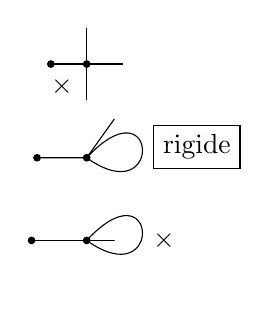
\begin{tikzpicture}[line cap=round,scale=.7]\fill(0,0)circle(2pt);\draw(0,0)--(90:.65);\draw(0,0)--(180:.65);\draw(0,0)--(270:.65);\draw(0,0)--(0:.65);\fill(-.65,0)circle(2pt);\node at(-.45,-.4){$\times$};\begin{scope}[shift={(0,-1.7)}]\fill(0,0)circle(2pt);\draw(0,0)..controls(1.3,1.4)and(1.4,-1)..(0,0);\draw(-.9,0)--(0,0)--(.5,.7);\fill(-.9,0)circle(2pt);\node[draw]at(2,.2){\uline{rigide}};\end{scope}\begin{scope}[shift={(0,-3.2)}]\fill(0,0)circle(2pt);\draw(0,0)..controls(1.3,1.4)and(1.4,-1)..(0,0);\draw(-1,0)--(.5,0);\fill(-1,0)circle(2pt);\node at(1.4,0){$\times$};\end{scope}\end{tikzpicture}}
c) $2$ sommets, d’ordre $3$ et $2$
\figure{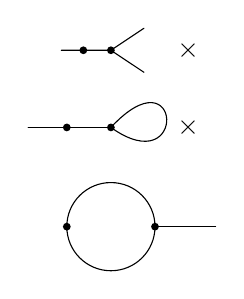
\begin{tikzpicture}[line cap=round,scale=.7]\fill(0,0)circle(2pt);\draw(-.9,0)--(0,0)--(.6,.4);\draw(0,0)--(.6,-.4);\fill(-.5,0)circle(2pt);\node at(1.4,0){$\times$};\begin{scope}[shift={(0,-1.4)}]\fill(0,0)circle(2pt);\draw(0,0)..controls(1.3,1.4)and(1.4,-1)..(0,0);\draw(-1.5,0)--(0,0);\fill(-.8,0)circle(2pt);\node at(1.4,0){$\times$};\end{scope}\begin{scope}[shift={(0,-3.2)}]\draw(0,0)circle(.8);\fill(-.8,0)circle(2pt);\fill(.8,0)circle(2pt);\draw(.8,0)--(1.9,0);\end{scope}\end{tikzpicture}}
d) $3$ sommets, dont $1$ d’ordre $3$, deux d’ordre $1$
\figure{\begin{tikzpicture}[line cap=round,scale=.7]\fill(0,0)circle(2pt);\draw(-.9,0)--(0,0)--(.6,.4);\draw(0,0)--(.6,-.4);\fill(-.9,0)circle(2pt);\fill(.6,-.4)circle(2pt);\node at(1.4,0){$\times$};\end{tikzpicture}}
e) $3$ sommets, \deleted{dont} $2$ d’ordre $2$, $1$ d’ordre $1$
\deleted{\figure{\begin{tikzpicture}[line cap=round,scale=.7]\fill(0,0)circle(2pt);\draw(0,0)..controls(1.3,1.4)and(1.4,-1)..(0,0);\draw(-.3,.5)--(.7,.6)--(0,-.2)--(1,0)--(.5,-.3);\end{tikzpicture}}}
\figure{\begin{tikzpicture}[line cap=round,scale=.7]\draw(-1,0)--(1.8,0);\foreach\a in{-1,0,1}\fill(\a,0)circle(2pt);\node at(2.3,0){$\times$};\end{tikzpicture}}
f) $4$ sommets, dont trois d’ordre $1$, $1$ d’ordre $2$\margin{impossible\ldots}

\scanpage{119}
% archive foliation: 118
\uline{degré $6$}\quad a) $1$ sommet d’ordre $6$
\figure{\begin{tikzpicture}[scale=.64,line cap=round,line join=round]\begin{scope}[shift={(6,3)}]\fill(0,0)circle(2pt);\draw(0,0)--(30:.8);\draw(0,0)--(90:.8);\draw(0,0)--(150:.8);\draw(0,0)--(210:.8);\draw(0,0)--(270:.8);\draw(0,0)--(330:.8);\node at(0,-1){$\uuline{D_6}$};\end{scope}\begin{scope}[shift={(9,3)}]\fill(0,0)circle(2pt);\draw(0,0)..controls(1.3,1.4)and(1.4,-1)..(0,0);\draw(-.7,.4)--(0,0)--(-.7,-.4);\draw(0,-.7)--(0,0)--(.4,-.6);\node at(0,-1){$\mathbb Z_2$};\end{scope}\begin{scope}[shift={(12,3)}]\fill(0,0)circle(2pt);\draw(0,0)..controls(1.3,1.4)and(1.4,-1)..(0,0);\draw(-.7,.2)--(0,0)--(.5,.1);\draw(-.5,-.6)--(0,0)--(0,-.7);\node at(0,-1){$\mathbb Z_2$};\end{scope}\begin{scope}[shift={(0,1.1)}]\fill(0,0)circle(2pt);\draw(0,0)..controls(1.3,1.4)and(1.4,-1)..(0,0);\draw(-.7,.3)--(0,0)--(.6,.2);\draw(-.7,-.4)--(0,0)--(.6,-.2);\node at(0,-1){$\mathbb Z_2\times\mathbb Z_2$};\end{scope}\begin{scope}[shift={(3.1,1.1)}]\fill(0,0)circle(2pt);\draw(0,0)..controls(-1.2,1.3)and(-1.5,-1.2)..(0,0)..controls(1.4,1.2)and(1.4,-1.2)..(0,0);\draw(-.6,-.6)--(0,0)--(0,-.8);\node at(0,-1){$\mathbb Z_2$};\end{scope}\begin{scope}[shift={(6.5,1.1)}]\fill(0,0)circle(2pt);\draw(0,0)..controls(-1.2,1.3)and(-1.5,-1.2)..(0,0)..controls(1.4,1.2)and(1.4,-1.2)..(0,0);\draw(.7,.2)--(0,0)--(.6,-.2);\node at(1.2,-.7){$\times$};\node at(0,-1){$\mathbb Z_2$};\end{scope}\begin{scope}[shift={(10,1.1)}]\fill(0,0)circle(2pt);\draw(0,0)..controls(-1.2,1.3)and(-1.5,-1.2)..(0,0)..controls(1.4,1.2)and(1.4,-1.2)..(0,0);\draw(-.7,0)--(.7,.2);\node at(0,-1){$\mathbb Z_2\times\mathbb Z_2$};\end{scope}\begin{scope}[shift={(0,-1.3)}]\fill(0,0)circle(2pt);\draw(0,0)..controls(-1.2,1.3)and(-1.5,-1.2)..(0,0)..controls(1.4,1.2)and(1.4,-1.2)..(0,0);\draw(0,.7)--(0,0)--(.7,0);\node at(-1.2,-.8){$\times$};\node[draw,circle]at(0,-1){$1$};\end{scope}\begin{scope}[shift={(3,-1.3)}]\fill(0,0)circle(2pt);\draw(0,0)..controls(-1.2,1.3)and(-1.5,-1.2)..(0,0)..controls(1.4,1.2)and(1.4,-1.2)..(0,0);\draw(0,0)..controls(-.5,-1.7)and(.6,-1.7)..(0,0);\node at(0,-1){$\mathfrak S_3$};\end{scope}\begin{scope}[shift={(6.5,-1.3)}]\fill(0,0)circle(2pt);\draw(0,0)..controls(-1.2,1.3)and(-1.5,-1.2)..(0,0)..controls(1.4,1.2)and(1.4,-1.2)..(0,0);\draw(0,0)..controls(1.1,.7)and(1.1,-.7)..(0,0);\node at(0,-1){$\mathbb Z_2$};\end{scope}\begin{scope}[shift={(10.6,-1.6)}]\fill(0,0)circle(2pt);\draw(0,0)..controls(-1.2,1.3)and(-1.5,-1.2)..(0,0)..controls(1.4,1.2)and(1.4,-1.2)..(0,0);\draw(0,-.8)--(0,.8);\node at(0,-1){$\mathbb Z_2\times\mathbb Z_2$};\end{scope}\draw(7.5,3.8)--(7,2.5);\draw(7.6,3.8)--(7.1,2.5);\draw(1.7,2)--(1.7,.3);\draw(1.8,2)--(1.8,.3);\draw(1.5,-.5)--(1.1,-2.3);\draw(1.6,-.5)--(1.2,-2.3);\draw(12.1,1.5)--(12.2,.1);\foreach\y in{.2,.4,...,1.5}\draw(12,\y)--(12.3,\y+.15);\draw(1.9,2.1)..controls(4,2.4)and(4,1.1)..(4.8,.4)..controls(7,-.2)and(9.8,-.3)..(11.5,-.3)..controls(12.7,-2.7)..(11.4,-2.7)--(9.3,-2.7)..controls(8.8,-2.7)and(9,-1.5)..(8.5,-1)..controls(7,.1)and(4,-.2)..(3,-.25)..controls(1.5,-.4)..(1.9,2.1);\node at(10.5,-3.4){$\left(6,\begin{smallmatrix}2_2\\1_2\end{smallmatrix},\begin{smallmatrix}\unsure4\\\unsure{1_2}\end{smallmatrix}\right)$};\end{tikzpicture}}
b) $1$ sommet d’ordre $5$, $1$ d’ordre $1$
\figure{\begin{tikzpicture}[scale=.64,line cap=round,line join=round]\begin{scope}[shift={(0,1.5)}]\fill(0,0)circle(2pt);\draw(-.8,0)--(0,0)--(.8,.5);\draw(0,-.7)--(0,.7);\draw(0,0)--(.8,-.2);\fill(-.8,0)circle(2pt);\node at(0,-1){$\mathbb Z_2$};\end{scope}\begin{scope}[shift={(3.3,1.5)}]\fill(0,0)circle(2pt);\draw(0,0)..controls(1.3,1.4)and(1.4,-1)..(0,0);\draw(-1,0)--(0,0)--(0,-.7);\draw(0,0)--(.4,-.7);\fill(-1,0)circle(2pt);\node at(0,-1){$\deleted{\unsure{\mathbb Z_2}}\quad1$};\end{scope}\begin{scope}[shift={(6.8,1.5)}]\fill(0,0)circle(2pt);\draw(0,0)..controls(1.3,1.4)and(1.4,-1)..(0,0);\draw(-1,0)--(.6,0);\draw(0,0)--(-.2,-.7);\fill(-1,0)circle(2pt);\node[draw,circle]at(0,-1){$1$};\end{scope}\begin{scope}[shift={(10.2,1.5)}]\fill(0,0)circle(2pt);\draw(0,0)..controls(1.3,1.4)and(1.4,-1)..(0,0);\draw(-1,0)--(0,0)--(.7,.2);\draw(0,0)--(.7,-.2);\fill(-1,0)circle(2pt);\node at(0,-1){$\mathbb Z_2$};\end{scope}\begin{scope}[shift={(0,-1.2)}]\fill(0,0)circle(2pt);\draw(-.9,0)--(0,0)..controls(.6,1.6)and(1.6,1.1)..(0,0)..controls(1.6,-.1)and(1.6,-1.5)..(0,0);\fill(-.9,0)circle(2pt);\node at(0,-1){$\mathbb Z_2$};\end{scope}\begin{scope}[shift={(3.3,-1.2)}]\fill(0,0)circle(2pt);\draw(0,0)..controls(.6,1.6)and(1.6,1.1)..(0,0)..controls(1.6,-.1)and(1.6,-1.5)..(0,0);\draw(0,0)--(.8,.5);\fill(.8,.5)circle(2pt);\node[draw,circle]at(0,-1){$1$};\end{scope}\begin{scope}[shift={(8,-1.6)}]\fill(0,0)circle(2pt);\draw(0,0)..controls(1.3,1.4)and(1.4,-1)..(0,0);\draw(-1,0)--(0,0)--(-.4,.5);\draw(0,0)--(-.4,-.5);\fill(-1,0)circle(1.5pt);\node at(0,-1){$\mathbb Z_2$};\end{scope}\draw(2,1.8)..controls(2,2.7)and(5,2.8)..(5,2)..controls(4.9,.7)and(8,.1)..(9,-.6)..controls(11,-2.7)and(7,-3.4)..(6,-1.5)..controls(5,.5)and(1.8,.7)..(2,1.8);\draw[->](4.3,.7)..controls(6,-.5)..(6.4,-1);\end{tikzpicture}}
c) $1$ sommet d’ordre $4$, $1$ d’ordre $2$
\figure{\begin{tikzpicture}[scale=.64,line cap=round,line join=round]\begin{scope}[shift={(0,0)}]\fill(0,0)circle(2pt);\draw(-1.5,0)--(.9,0);\draw(.8,.6)--(0,0)--(.8,-.6);\fill(-.8,0)circle(2pt);\node at(0,-1){$\mathbb Z_2$};\end{scope}\begin{scope}[shift={(4,0)}]\fill(0,0)circle(2pt);\draw(0,0)..controls(1.3,1.4)and(1.4,-1)..(0,0);\draw(-1.5,0)--(0,0)--(.6,-.7);\fill(-.8,0)circle(2pt);\node[draw,circle]at(0,-1){$1$};\end{scope}\begin{scope}[shift={(8,0)}]\fill(0,0)circle(2pt);\draw(0,0)..controls(1.3,1.4)and(1.4,-1)..(0,0);\draw(-1.5,0)--(.5,0);\fill(-.8,0)circle(2pt);\node at(0,-1){$\mathbb Z_2$};\end{scope}\end{tikzpicture}}
\margin{\figure{\begin{tikzpicture}[scale=.64,line cap=round,line join=round]\begin{scope}[shift={(-1,1.7)}]\fill(0,0)circle(2pt);\draw(0,0)..controls(1.3,1.4)and(1.4,-1)..(0,0);\draw(-.6,0)--(.4,0);\fill(.9,.2)circle(1.5pt);\node at(-.7,.6){$(\alpha)$};\node at(0,-1){$\mathbb Z_2$};\end{scope}\begin{scope}[shift={(1.6,1.7)}]\fill(0,0)circle(2pt);\draw(0,0)..controls(1.3,1.4)and(1.4,-1)..(0,0);\draw(-.5,.3)--(0,0)--(-.5,-.3);\fill(.9,.2)circle(1.5pt);\node at(-.7,.6){$(\gamma)$};\node at(0,-1){$\mathbb Z_2$};\end{scope}\begin{scope}[shift={(-1,-0.4)}]\fill(0,0)circle(2pt);\draw(0,0)..controls(-1.2,1.3)and(-1.5,-1.2)..(0,0)..controls(1.4,1.2)and(1.4,-1.2)..(0,0);\fill(-.9,0)circle(1.5pt);\node at(-1.2,.6){$(\beta)$};\node at(0,-1){$\mathbb Z_2$};\end{scope}\end{tikzpicture}}}
d) $1$ sommet d’ordre $4$, deux d’ordre $1$
\figure{\begin{tikzpicture}[scale=.64,line cap=round,line join=round]\begin{scope}[shift={(0,0)}]\fill(0,0)circle(2pt);\foreach\a in{45,135,225,315}\draw(0,0)--(\a:.8);\fill(45:.8)circle(2pt);\fill(135:.8)circle(2pt);\node at(0,-1){$\mathbb Z_2$};\end{scope}\begin{scope}[shift={(3,0)}]\fill(0,0)circle(2pt);\draw(-.6,.6)--(0,0)--(.6,.6);\fill(-.6,.6)circle(2pt);\fill(.6,.6)circle(2pt);\draw(0,0)..controls(-1,-1.6)and(1,-1.6)..(0,0);\node at(0,-1){$\mathbb Z_2$};\end{scope}\begin{scope}[shift={(5.7,0)}]\fill(0,0)circle(2pt);\draw(0,0)--(90:.65);\draw(0,0)--(180:.65);\draw(0,0)--(270:.65);\draw(0,0)--(0:.65);\fill(-.65,0)circle(1.5pt);\fill(.65,0)circle(1.5pt);\node at(-.9,.6){$(\delta)$};\node at(0,-1){$\mathbb Z_2\times\mathbb Z_2$};\end{scope}\begin{scope}[shift={(8.3,0)}]\fill(0,0)circle(2pt);\draw(0,0)..controls(-1.3,1.4)and(-1.4,-1)..(0,0);\draw(-.5,0)--(.5,0);\fill(-.5,0)circle(1.5pt);\fill(.5,0)circle(1.5pt);\node at(-.8,.6){$(\unsure{\eta})$};\node at(0,-1){$\mathbb Z_2$};\end{scope}\end{tikzpicture}}
e) $2$ sommets d’ordre $3$\margin{$\deleted{\unsure2}$}
\deleted{\figure{\begin{tikzpicture}[scale=.64,line cap=round,line join=round]\begin{scope}[shift={(0,0)}]\draw(0,0)--(1.2,0);\draw(0,0)..controls(-1.4,1.4)and(-1.4,-1.2)..(0,0);\draw(1.2,0)..controls(2.6,1.4)and(2.6,-1.2)..(1.2,0);\fill(0,0)circle(2pt);\fill(1.2,0)circle(2pt);\foreach\x in{-.7,-.5,...,2}\draw(\x,-.6)--(\x+.7,.8);\node at(0,-1){$\mathbb Z$};\end{scope}\end{tikzpicture}}}
\figure{\begin{tikzpicture}[scale=.64,line cap=round,line join=round]\begin{scope}[shift={(7,1)}]\draw(0,0)--(1.2,0);\draw(0,0)..controls(-1.4,1.4)and(-1.4,-1.2)..(0,0);\draw(1.2,0)..controls(2.6,1.4)and(2.6,-1.2)..(1.2,0);\fill(0,0)circle(2pt);\fill(1.2,0)circle(2pt);\node at(0,-1){$\mathbb Z_2\times\mathbb Z_2$};\end{scope}\begin{scope}[shift={(2,-1.4)}]\fill(0,0)circle(2pt);\draw(0,0)..controls(-1.3,1.4)and(-1.4,-1)..(0,0);\draw(0,0)--(1.2,0)--(1.8,.5);\draw(1.2,0)--(1.8,-.5);\fill(1.2,0)circle(2pt);\node at(0,-1){$\mathbb Z_2$};\end{scope}\begin{scope}[shift={(7,-1.4)}]\draw(-.7,.5)--(0,0)--(-.7,-.5);\draw(0,0)--(1,0);\draw(1.7,.5)--(1,0)--(1.7,-.5);\fill(0,0)circle(2pt);\fill(1,0)circle(2pt);\node at(0,-1){$\mathbb Z_2\times\mathbb Z_2$};\end{scope}\end{tikzpicture}}
\figure{\begin{tikzpicture}[scale=.64,line cap=round,line join=round]\begin{scope}[shift={(0,0)}]\draw(0,0)..controls(.6,.8)and(1.1,.8)..(1.5,0)..controls(1,-.8)and(.4,-.8)..(0,0);\fill(0,0)circle(2pt);\fill(1.5,0)circle(2pt);\draw[thick](0,0)--(1.5,0);\node at(0,-1){$\mathbb Z_2.\mathfrak S_3\quad\deleted{\unsure{D_3\times\mathbb Z_2}}$};\end{scope}\begin{scope}[shift={(4,0)}]\draw(0,0)..controls(.6,.8)and(1.1,.8)..(1.5,0)..controls(1,-.8)and(.4,-.8)..(0,0);\fill(0,0)circle(2pt);\fill(1.5,0)circle(2pt);\draw(-.6,0)--(0,0);\draw(1.5,0)--(2.1,0);\node at(0,-1){$\mathbb Z_2\times\mathbb Z_2$};\end{scope}\begin{scope}[shift={(8,0)}]\draw(0,0)..controls(.6,.8)and(1.1,.8)..(1.5,0)..controls(1,-.8)and(.4,-.8)..(0,0);\fill(0,0)circle(2pt);\fill(1.5,0)circle(2pt);\draw(0,0)--(.6,0);\draw(1.5,0)--(2.1,0);\node at(0,-1){$\mathbb Z_2\times\mathbb Z_2$};\end{scope}\end{tikzpicture}}

\scanpage{120}
% archive foliation: 119
f) $1$ sommet d’ordre $3$, $1$ d’ordre $2$, $1$ d’ordre $2$
\figure{\begin{tikzpicture}[scale=.64,line cap=round,line join=round]\begin{scope}[shift={(0,1)}]\fill(0,0)circle(2pt);\draw(0,.7)--(0,-.7);\draw(0,0)--(1.3,0);\fill(0,-.7)circle(2pt);\fill(.65,0)circle(2pt);\node at(.9,.55){$\times$};\node[draw,circle]at(0,-1){$1$};\end{scope}\begin{scope}[shift={(3,1)}]\fill(0,0)circle(2pt);\draw(-.8,.4)--(0,0)--(1,.6)--(2,.5);\draw(0,0)--(0,-.8);\fill(0,-.8)circle(2pt);\fill(1,.6)circle(2pt);\draw(1,.6)--(1.5,1.2);\node[draw,circle]at(0,-1){$1$};\end{scope}\begin{scope}[shift={(6.8,1)}]\fill(0,0)circle(2pt);\draw(-.5,.7)--(0,0)--(-.5,-.7);\draw(0,0)--(2,0);\fill(1,0)circle(2pt);\fill(2,0)circle(2pt);\node at(.8,.65){$\times$};\node at(0,-1){$\mathbb Z_2$};\end{scope}\begin{scope}[shift={(0,-1.5)}]\fill(0,0)circle(2pt);\draw(0,0)..controls(1.3,1.4)and(1.4,-1)..(0,0);\draw(-.6,.6)--(0,0)--(-.6,-.5);\fill(-.6,.6)circle(2pt);\fill(.95,.1)circle(2pt);\end{scope}\begin{scope}[shift={(3,-1.5)}]\fill(0,0)circle(2pt);\draw(0,0)..controls(1.3,1.4)and(1.4,-1)..(0,0);\draw(-.7,.5)--(0,0)--(-.7,-.5);\draw(0,0)--(1,0);\fill(1,0)circle(2pt);\node at(0,-1){$\unsure{1}\quad\mathbb Z_2$};\end{scope}\begin{scope}[shift={(6.8,-1.5)}]\fill(0,0)circle(2pt);\draw(0,0)..controls(-1.3,1.4)and(-1.4,-1)..(0,0);\draw(0,0)--(1.6,0);\fill(.7,0)circle(2pt);\node at(0,-1){$\mathbb Z_2$};\end{scope}\draw(2,2)--(1.8,-1.8);\draw(3.8,2)--(3.4,-1.6);\draw(4.7,2)--(4,-1.9);\draw(2,-1.5)..controls(3,-4)and(4,-2.5)..(4.6,-1.4)..controls(5.1,-.4)and(4.4,-.7)..(4,-1.6);\draw(2.7,-1.7)circle(.4);\draw(2.3,-1.3)--(3.1,-2.1);\draw(3.1,-1.3)--(2.3,-2.1);\end{tikzpicture}}
\margin{$\left(\begin{smallmatrix}3\\2\\1\end{smallmatrix},\begin{smallmatrix}2_2\\1_2\end{smallmatrix},\unsure6\right)$\\$\left(\begin{smallmatrix}3\\2\\1\end{smallmatrix},\begin{smallmatrix}2_2\\1_2\end{smallmatrix},\unsure6\right)$\\$\left(\begin{smallmatrix}3\\2\\1\end{smallmatrix},\unsure{2_3},\begin{smallmatrix}5\\1\end{smallmatrix}\right)$\\$\left(\begin{smallmatrix}3\\2\\1\end{smallmatrix},2_3,\begin{smallmatrix}4\\2\end{smallmatrix}\right)$}
\figure{\begin{tikzpicture}\draw(0,0)..controls(.1,.7)and(.6,.8)..(.8,.8)--(.8,1.3);\draw(.9,.8)..controls(1.2,.4)and(2,.7)..(2.7,0);\draw(1.4,2.6)..controls(.8,2.4)..(1,2.1);\end{tikzpicture}}
g) $1$ sommet d’ordre $3$, \unsure{trois} d’ordre $1$
\figure{\begin{tikzpicture}[scale=.64,line cap=round,line join=round]\begin{scope}[shift={(0,0)}]\fill(0,0)circle(2pt);\draw(0,0)--(90:.65);\draw(0,0)--(210:.65);\draw(0,0)--(330:.65);\foreach\a in{90,210,330}\fill(\a:.65)circle(2pt);\node at(0,-1){$\uuline{D_3}$};\end{scope}\end{tikzpicture}}
\deleted{\figure{\begin{tikzpicture}[scale=.64]\fill(0,0)circle(2pt);\draw(0,0)--(90:.65);\draw(0,0)--(210:.65);\draw(0,0)--(330:.65);\draw(-.2,.8)--(.5,.6)--(-.3,.1)--(.5,0)--(-.3,-.5)--(.2,-.5);\end{tikzpicture}}}
\[\left(\begin{smallmatrix}3\\1_3\end{smallmatrix},2_3,6\right)\]
h) $3$ sommets d’ordre $2$
\figure{\begin{tikzpicture}[scale=.64,line cap=round,line join=round]\begin{scope}[shift={(0,0)}]\draw(0,0)circle(.8);\foreach\a in{90,180,320}\fill(\a:.8)circle(2pt);\node at(0,-1){$\uline{\mathbb Z_2.\unsure{D_3|\mathfrak S_3}}$};\end{scope}\begin{scope}[shift={(3.5,0)}]\draw(-1.4,0)--(1.4,0);\foreach\x in{-.7,0,.7}\fill(\x,0)circle(1.5pt);\node at(0,-1){$\mathbb Z_2\times\mathbb Z_2$};\end{scope}\end{tikzpicture}}
\margin{$\left(2_3,2_3,3_2\right)$\\$\left(2_3,\begin{smallmatrix}2_2\\1_2\end{smallmatrix},6\right)$}
i) $2$ sommets d’ordre $2$, $2$ d’ordre $1$
\figure{\begin{tikzpicture}[scale=.64,line cap=round,line join=round]\begin{scope}[shift={(0,0)}]\draw(-1.2,0)--(1.2,0);\foreach\x in{-1.2,-.4,.4,1.2}\fill(\x,0)circle(2pt);\node at(0,-1){$\mathbb Z_2\times\mathbb Z_2$};\end{scope}\end{tikzpicture}}
\[\left(\begin{smallmatrix}2_2\\1_2\end{smallmatrix},2_3,6\right)\]
j) $1$ sommet d’ordre $2$, $4$ d’ordre $1$
\figure{\begin{tikzpicture}\draw(0,0)--(.9,0);\fill(0,0)circle(1pt);\fill(.9,0)circle(1pt);\node[draw,ellipse]at(3,.3){impossible};\end{tikzpicture}}

\scanpage{121}
% archive foliation: 120
\margin{``Opérations'' sphériques\\sur les cartes\\(axiomatique provisoire)}
\figure{\begin{tikzpicture}\draw(0,0)--(.2,.04);\end{tikzpicture}}

\scanpage{122}
% archive foliation: 121
$1.$ \deleted{Appelons ``opération'' (sur cartes) \unsure{toute|tout}}
\deleted{Soit $C=(X,K,S)$ une carte \inserted{orientée}}, soit $F$ un \deleted{foncteur}\inserted{foncteur} sur la catégorie des
\deleted{surfaces compactes (avec comme morphismes les morphismes de revêtement (avec ramification))}
\inserted{cartes finies orientées}.
[On suppose que si $(X,H)$ est une surface compacte avec $H$ groupe fini opérant avec ramification isolée, on a
\[
F(X/H)=F(X)^H.
\]
]
$\operatorname{Aut}(C)$ opère sur $F(X)$, donc et son sous-groupe $N(C)\inserted{=\operatorname{Aut}^\circ(C)}$ des autom. isotopes à l’identité.
\margin{On suppose que \unsure{les foncteurs} \unsure{seront tous} \unsure{contravariants}.}
\unsure{Quoi|Puis}, soit
\[
F^{\unsure{\natural|\sharp}}(C)=F(X)/\operatorname{Aut}^\circ(C).
\]
C’est un \deleted{foncteur}\inserted{préfaisceau} en $C$, car si
\[
C'=(X',K',S')\xrightarrow{f}(X,K,S),
\]
on a $F(X)\to F(X')$ \deleted{et $\unsure{\operatorname{Aut}(f)}\operatorname{Aut}(f)^\circ$}
en façon compatible avec $\operatorname{Aut}(f)^\circ$, donc
\[
F(X)/\operatorname{Aut}(f)^\circ\longrightarrow F(X')/\operatorname{Aut}(f)^\circ,
\]
par $\operatorname{Aut}(f)^\circ\xrightarrow{\sim}\operatorname{Aut}(X)^\circ$ d’où par composition
\[
F(X)/\operatorname{Aut}(C)^\circ\longrightarrow F(X')/\operatorname{Aut}(f)^\circ
\longrightarrow F(X')/\operatorname{Aut}(C')^\circ
\]
i.e. $F^\natural(C)\to F^\natural(C')$.
On étend $F^\natural$ en un foncteur sur la catégorie des cartes finies $C$ avec groupe fini d’autom., en posant
\[
F^\natural(C,G)=F(C)^G/\operatorname{Aut}(C,G)^\circ.
\]
Ceci dit, on se propose de trouver les sections de \deleted{\unsure{ce $F$}}
\[
F^\natural:\underset{\text{finies}}{\text{Cartes}}\ \text{à opérateurs}\ \inserted{\text{finis}}\longrightarrow\text{ens}
\]

\scanpage{123}
% archive foliation: 122
Un argument \unsure{assez} formel montre que
\[
\Gamma(F^\natural)\simeq\underset{H_\alpha}{\varinjlim}\ F^\natural(C_\alpha,G_\alpha)
\]
\deleted{où $\unsure{G_\alpha},C_\alpha$}
où $H_\alpha$ parcourt les sous-groupes \uline{inv} d’indice fini du groupe cartographique orienté, $C_\alpha$ est la carte orientée associée à $H_\alpha$, $G_\alpha=\mathbb G_2^+/H_\alpha$.
\uline{Ex} Soit $F(C)=\mathcal P(X)$, alors
\[
\Gamma F^\natural\simeq\mathcal P(S)/\operatorname{Aut}^\circ(S,
\]
$S$ \unsure{est} la sphère munie du segment $[0,1]$ et du point $\infty$,
\deleted{\unsure{pointée en $(0,1,\infty)$}} qui sert de référence dans notre théorie de cartographie.
\figure{\begin{tikzpicture}[scale=.8]
\draw(0,0)ellipse(1.2 and1.3);\draw[dashed](-1.2,0)..controls(-.4,.6)and(.5,.6)..(1.2,.15);
\draw[dashed](-1.2,0)..controls(-1,-.35)..(-.7,-.3);
\draw[very thick](-.7,-.3)..controls(.4,-.4)..(1.2,.15);
\draw(-.7,-.3)..controls(-.4,.2)and(.3,.3)..(1.2,.15);
\fill(-.7,-.3)circle(2pt)node[below]{$0$};\fill(1.2,.15)circle(2pt)node[right]{$1$};\fill(0,.4)circle(2pt)node[right]{$\infty$};
\end{tikzpicture}}
\uline{NB} Si on avait pris la théorie non orientée, on aurait trouvé
\[
\Gamma(F^\natural)\simeq\mathcal P(S)^{\uline c}/
\underbrace{\operatorname{Aut}(S,\uline c,0,1,\infty)^\circ}_{\simeq\operatorname{Aut}(S^+,0,1,\infty)^\circ}
\]
où $\uline c$ est la conjugaison (ayant comme pts fixes l’``équateur'' qui passe par $0,1,\infty\ldots$)
\uline{NB} On prouve \inserted{\unsure{aussitôt}} que, pour que \deleted{\unsure{notre}}\inserted{la} section $\Omega$ de $F^\natural$ \deleted{\unsure{associée}}\inserted{définie}: une partie \inserted{$A$} de $S$ \deleted{définie}\inserted{associe} \deleted{\unsure{, puis à}} à toute carte $C=(X,K,S)$ \deleted{des} parties \inserted{$A_X$} de $X$ qui \deleted{\unsure{sont}} un sous-$1$-complexe topologique, il f. et s. que la partie de $S$ envisagée soit de $=$ \unsure{nature}.
\figure{\begin{tikzpicture}
\draw(0,0)--(1.7,.25)--(1.65,1.6)--(.3,1.5)--(-.25,.85)--cycle;
\draw[thick](0,0)--(.7,.8)--(1.65,1.6);\draw(.3,1.5)--(.7,.8)--(1.7,.25);\draw(-.25,.85)--(.7,.8);
\draw[very thick](0,0)--(1.7,.25)--(1.65,1.6);\end{tikzpicture}}
Pour que les $A_X\cup K$ soient des sous-$1$-complexes (pas de \unsure{somm.-gén.|somm. qui}) \unsure{cf] et 1|si] et 1}.

\scanpage{124}
% archive foliation: 123
(auquel cas les pts correspondants des
$A_X$ \uline{ne sont pas} des sommets topologiques
\unsure{\ldots}) \deleted{\unsure{on}} \deleted{\unsure{en}} \inserted{\unsure{se permet de}}
\unsure{le considère|les considère} comme un ``milieu
d'arête'' des $A_X$.

À l'exclusion de ce cas, on peut dire
que $A$, avec l'ens de ses sommets
choisis (qui \unsure{c.} \deleted{\unsure{A}} \uline{tous} \uline{les} sommets
topologiques, et les pts $0,1,\infty$ \inserted{qui sont $\in A$}, (qu'ils
\unsure{soient ou non} sommets top., et éventuellement
$N$ autres, \unsure{enfin} suivant l'opération
qu'on veut obtenir sur les sommets
qu'on entend donner aux $A_X$), et
le choix des centres des faces fait
en conformité avec la condition $1^\circ$,
et enfin un choix \uline{arbitraire} des
milieux d'arête de $A$ (tous distincts
\unsure{même} de $0,1,\infty$) est \unsure{déduit} d'une
application $\varphi:S\to S$ ramifiée aux
seuls pts $0,1,\infty$, avec ramification
$2$ au dessus de $1$, en prenant l'image
inverse de $[0,1]$ -- et l'image inverse
\deleted{dans} $A_X$ dans $X$ par $f:X\to S$ de
$A$ n'est que $(\varphi f)^{-1}([0,1])$,
\unsure{où} $\varphi f$ est \deleted{ramifiée} un rev. \unsure{en dehors de}
$0,1,\infty$ (car $\varphi^{-1}\{0,1,\infty\}\supset\{0,1,\infty\}$ et

\scanpage{125}
% archive foliation: 124
que $A\cup[0,1]$ soit un $1$-complexe.

Pour que de plus les $A_X$ \deleted{\unsure{soient définis}}\inserted{\unsure{définissent}}
sur les $X$ de nouvelles structures de
Cartes (i.e. $X\setminus A_X$ a comp. conn. $\simeq$ disques)
il f. et s. que a) $A_{\unsure X}$ soit connexe
\deleted{\unsure{Ou si $A$ ne l'est plus}}\par
\deleted{b) $A$ contienne deux des pts $0,1,\infty$ (\unsure{ou au moins}}\par
\deleted{\unsure{s'il laisse plus des pts $0,1,\infty$ qui ne $\in A$})}\par
\deleted{\unsure{ou bien}}\par
\inserted{i.e. définisse une carte sur $S^1$}

b) \deleted{\unsure{À une face}} \unsure{aucune des} \deleted{\unsure{deux}} \unsure{cette carte|dites cartes}
ne peut contenir au plus qu'un seul
des pts $0,1,\infty$.

Supposons cette condition satisfaite. Choisissons
des sommets de $A$, \deleted{\unsure{et}} des centres des
faces, des milieux d'arêtes, de façon
à satisfaire à $2$ conditions:

$1^\circ)$ Si \deleted{\unsure{un}} des pts $0,1,\infty$ est dans une
face ouverte, on le choisit comme
centre de la dite [il n'y a pas de conflit\ldots]

$2^\circ)$ Sinon (i.e. \deleted{\unsure{s'il est}} $s\in A$] on choisit $s$
comme un sommet de $A$, \deleted{\unsure{à}} à l'exception
du seul cas qui suit:
\margin{\unsure{on n'est pas obligé de faire}, \unsure{i.e.} \unsure{choisir tous les sommets topolog. des $A_X$}\ldots}

$3^\circ)$ Si $s=1\in A$, et si $s$ est \deleted{un} \inserted{un} pt
d'ordre $1$ de $A$\par
i.e. un bout
\figure{\begin{tikzpicture}[x=1cm,y=1cm]
\draw (0,0)--(2.1,0)--(2.5,.45);
\draw (2.1,0)--(2.5,-.5)--(3,-.43) .. controls (3.05,.9) and (4,.65) .. (4,-.35) .. controls (3.9,-.65) and (3.15,-.7) .. (3,-.43);
\draw (0,0) circle (.045);\node[below] at (0,0) {$s$};\node[below] at (1.2,0) {$A$};
\end{tikzpicture}}

\scanpage{126}
% archive foliation: 125
\uline{Th.} Soit $C=(X,\inserted{K,S})$ carte \uuline{connexe},
$G$ un groupe opérant \inserted{fidèlement} sur $X$\par
\deleted{Supposons que $G\to\operatorname{Aut}_{\mathrm{isot}}(C)$ soit injectif} \unsure{sur la carte}

Conditions équivalentes

a) \deleted{\unsure{L'inject. de $G$}} Pour $g\in G$ tel que $g_X$ soit isotope à id
(en tant qu'autom. de carte), $g_X=\operatorname{id}_X$, i.e. $g\unsure{=|\in}1$; i.e.
\inserted{$G\to\operatorname{Aut}_{\mathrm{isot}}(C)$ est injectif (i.e. $G$ opère fid. sur $X$ de $C$ à isotopie)}

\deleted{b) Pour ts (\unsure{mil.} d'arête, sommet) de $X$}\par
\deleted{Le stabilisateur dans $G$ est fini}
\inserted{b) Le noyau de $G\to\operatorname{Aut}_{\mathrm{isot}}(C)$ est fini.}
\figure{\begin{tikzpicture}[x=1cm,y=1cm]
\draw[->] (0,1.5)..controls(-.8,1.2)and(-.8,.4)..(0,0);
\draw[->] (0,1.5)--(.8,1.5);\draw[->] (0,0)--(.7,0);
\draw (-.15,-.2)rectangle(.8,.2);\node at (.15,1.65){$\unsure{b}$};\node at (.12,-.03){$\unsure{a}$};
\end{tikzpicture}}

c) Il existe une rigidification de $X$ invariante par $G$

\inserted{d) $(C,G)$ est isomorphe à la réalisation top. d'une op. de $G$ sur une carte combin.}

\inserted{Quand ces conditions sont remplies,}
\deleted{De plus,} l'espace des rigidifications de $X$ invariantes
par $G$ est contractile.

\[
a)\Longrightarrow b)\Longrightarrow c)\qquad\text{évident}
\]
\[
b)\Longrightarrow a)\quad\text{Revient à ceci:}
\]
\figure{\begin{tikzpicture}[x=1cm,y=1cm]
\draw (-.8,.1)--(-.5,1.1)--(.65,1.6);
\draw (.8,1.55)--(1.85,.55);\draw(1.9,.45)--(1.8,-.65);
\draw(1.7,-.85)--(.7,-1.6);\draw(.6,-1.45)--(-.4,-1.2);
\draw(-.5,-1.1)--(-.85,-.2);\draw(-.2,1.3)--(.45,1.6);\fill(.5,0)circle(.04);
\end{tikzpicture}\quad
\begin{tikzpicture}[x=1cm,y=1cm]
\draw(0,0)circle(1.3);\fill(-.6,1.15)..controls(.2,1.5)and(.5,1.2)..(.7,1.1)--(.3,.9)--(.2,.3)--(.1,.35)--(.1,1)--cycle;
\draw (-.55,.1)..controls(-.6,1.1)and(.5,1)..(.7,.2)..controls(.9,-.7)and(-.55,-.8)..(-.55,.1);
\draw(-.7,.3)--(-.95,-.1)--(-.7,-.6)--(.6,-.6)--(.55,.5)--(-.3,.6)--(-.7,.3);
\draw(0,.6)ellipse(.65 and .4);\draw(-.25,-.1)ellipse(.7 and .6);\draw(.2,.1)circle(.55);\draw(-.5,-.1)..controls(.7,.9)and(.5,-.9)..(-.5,-.1);
\draw[line width=1pt](.2,.7)..controls(.9,.6)and(.8,-.2)..(.2,-.05)..controls(-.1,.1)and(0,.5)..(.2,.7);
\end{tikzpicture}}

Si un groupe \uline{fini}
opère \inserted{fid.} sur une carte, par
des opérations isotopes à id, il opère trivialt.
Ou encore: si un autom. d'ordre fini est
isotop. à id, \deleted{il opère tr.} c'est id. Il suffit de
le voir pour un disque fermé et un pt sur
le \inserted{bord du} disque -- on voit d'abord que c'est l'identité
sur le bord, \deleted{\unsure{par}} soit
\figure{\begin{tikzpicture}[x=1cm,y=1cm]
\draw[thin](0,0)circle(1.65);
\draw[line width=1.1pt](-.7,.15)--(-.25,.7)--(.5,.65)--(.25,-.35)--(-.35,-.3)--(-.5,0)--cycle;
\draw[line width=1.1pt](-.25,.7)--(-.1,1.5)..controls(.2,1.65)and(.5,1.6)..(.65,1.5)--(.5,.65);
\draw(.7,1.5)--(1.2,1.3)--(.62,1.05);\draw(1.2,1.3)--(1.4,.7);\draw(1.2,1.3)--(1.6,1);
\draw[line width=1.3pt](.75,.2)ellipse(.42 and .5);\draw(.75,.2)ellipse(.35 and .45);\fill(.78,.2)ellipse(.08 and .14);\fill(-.15,.3)circle(.02);
\end{tikzpicture}\par
\begin{tikzpicture}[x=1cm,y=1cm]
\draw(0,0)circle(.45);\draw(-.7,0)--(.9,0);\draw[line width=1pt](0,0)--(.9,0);\fill(0,0)circle(.04);
\foreach \x in {-.05,.08,.21,.34,.47}{\draw[thin](\x,.15)--(\x+.17,.5);}
\end{tikzpicture}}

\scanpage{127}

% archive foliation: 126

\[
\deleted{(0,1)\to\infty}\quad (0,1)\to\unsure{\infty}\qquad (\infty,\tfrac12)\to0
\]
\[
\deleted{\frac{\unsure{az+b}\,(\unsure{c+d})z}{cz+d}}\quad\deleted{\unsure{az+d}}
\qquad z\mapsto\frac{\unsure{az|z}}{cz+(\unsure{d|1}-c)}
\]
\[
z\longrightarrow\frac{z\deleted{\unsure{+c-1}}}{cz+(1-c)}
\qquad\frac{z}{cz+(1-\unsure{z|c})}:\bigl(\frac{cz}{cz+1-c}+
\]

\figure{\begin{tikzpicture}[x=1cm,y=1cm]
\node at (0,0){$\uline{\infty}$};\draw[->](0,.1)--(.6,.9);\draw(0,.1)--(.3,.7);\draw[->](0,.1)..controls(.3,.1)and(.6,.5)..(.8,.5);
\end{tikzpicture}}

\figure{\begin{tikzpicture}[x=1cm,y=1cm]
\draw(0,0)ellipse(.85 and 1.25);\draw(.1,1.25)..controls(1.1,1.2)and(1.05,-1.2)..(.15,-1.25);
\draw(-.15,1.2)..controls(-.55,.75)and(-.5,.3)..(-.5,.15);\draw(-.5,-.3)..controls(-.5,-.85)and(-.2,-1.15)..(-.1,-1.25);
\fill(-.15,1.2)circle(.05);\fill(-.5,.15)circle(.035);\draw(-.1,-1.25)circle(.05);
\node[above]at(-.15,1.2){$0$};\node[below]at(-.1,-1.25){$1$};\node[left]at(-.5,.15){$\infty$};\node at(.55,.3){$\tfrac12$};
\end{tikzpicture}}

\figure{\begin{tikzpicture}[x=1cm,y=1cm]
\draw[line width=1pt](0,0)--(2.1,2.05)--(2.75,.1)--cycle;
\draw(1.7,.03)--(1.53,.45)--(1.7,.65)--(1.72,1.45)..controls(1.8,1.9)and(2.3,1.7)..(2.05,1.4)..controls(1.9,1.2)and(1.7,1.35)..(1.72,1.45);
\draw(1.3,.15)ellipse(.16 and .11);\draw(1.3,.35)--(1.6,.7);\draw(1.4,.58)--(1.55,.4);\draw(1.55,.95)--(1.75,.6);
\draw(2.02,.25)ellipse(.15 and .1);\draw(1.9,.4)--(2.15,.65)--(2.2,.95);\draw(2.15,.65)--(2.2,.5);\draw(1.8,.9)--(2.4,1.3);
\end{tikzpicture}}

\figure{\begin{tikzpicture}[x=1cm,y=1cm]
\draw(0,0)--(2,2)--(3.25,.12)--cycle;
\draw(1.1,1.1)..controls(1.85,.9)and(1.8,1.65)..(1.65,1.65);
\draw(1.65,1.65)--(2,1.9);\draw(1.7,1.57)--(2.1,1.8);\draw(1.75,1.4)--(2.15,1.38);\draw(1.55,1.05)--(1.65,.8);
\draw(1.15,1.02)--(.45,.2);\draw(1.2,1)--(.6,.16);\draw(1.3,1)--(1.05,.3);
\draw(1.8,.6)ellipse(.18 and .25);\draw(1.85,1.02)circle(.12);\draw(1.8,.85)--(1.85,.9);\draw(1.72,.35)--(1.6,.05);\draw(1.9,.35)--(1.95,.05);\draw(1.6,.6)--(1.4,.6);\draw(2,.6)--(2.15,.6);\draw(1.7,1.03)--(2,1.03);
\draw[rotate around={30:(2.55,.85)}](2.55,.85)ellipse(.12 and .36);\draw(2.4,1.16)..controls(2.2,1.4)and(2.2,1.1)..(2.4,1.16);\draw(2.63,.51)--(2.9,.3);\draw(2.65,1.05)--(2.8,1.25);\draw(2.75,.92)--(2.93,1.05);\draw(2.8,.78)--(3,.85);
\end{tikzpicture}}

\[
\begin{pmatrix}1&0\\c&1-c\end{pmatrix}
\begin{pmatrix}1&\unsure{0}\\c&1-c\end{pmatrix}
\quad\begin{pmatrix}1&0\\2c-c^2&(1-c)^2\end{pmatrix}
\]
\[
(1-c)^2=1\qquad\deleted{\unsure{c}}\qquad c-1=\pm1\qquad c=0\text{ ou }2
\]

\figure{\begin{tikzpicture}[x=1cm,y=1cm]
\draw(0,0)circle(1.2);\draw(-1.2,-.1)..controls(-.7,-.65)and(.6,-.6)..(1.18,-.1);\draw[dashed](-1.2,-.1)..controls(-.7,.65)and(.8,.6)..(1.18,-.1);
\draw(.2,1.18)..controls(.6,.6)and(-.05,.25)..(-.72,-.35);\draw(-.9,.4)--(-.72,-.35)--(-.15,.12);\draw(-.9,-.65)--(-.72,-.35);
\fill(-.72,-.35)circle(.05);\fill(.65,-.4)circle(.04);\fill(.4,.3)circle(.04);\node[above]at(-.65,1.02){$0$};\node[below]at(-.72,-.35){$p$};\node[below]at(.65,-.4){$1$};\node[right]at(.4,.3){$\infty$};\node at(.58,.75){$z$};
\end{tikzpicture}}

\figure{\begin{tikzpicture}[x=1cm,y=1cm]
\draw(-1.1,.7)..controls(-1.6,.55)and(-1.6,.4)..(-1.1,.45)--(.6,.55)..controls(1.6,.7)and(1.4,.8)..(.6,.8);
\draw(-1.1,.6)--(-1.1,1.1)..controls(-1.1,1.7)and(0,1.85)..(0,1.1)--(.05,.75)--(.25,.75);
\draw(-.85,.4)--(-.88,.05)--(-1,.0)--(-.75,-.03)--(-.68,-.13)--(-.75,-.2)--(-.55,-.24)--(-.6,-.34)--(-.43,-.4)--(-.43,-.55);
\draw(-.5,.35)--(.25,.45)--(.08,-.35)..controls(.6,.0)and(.9,.1)..(1.3,.15);
\draw(1.35,.1)..controls(1.8,.0)and(2,-.5)..(1.9,-.7);\draw(1.3,.15)--(.95,-.7);\draw(-.45,-.7)..controls(-.9,-1.2)and(-.2,-1.8)..(-.2,-1.8);\draw(.8,-1.2)--(2,-.9);
\draw(-.62,.3)--(-.5,.0)--(-.4,.2)--(-.65,.25)--(-.45,.05);
\end{tikzpicture}}

\figure{\begin{tikzpicture}[x=1cm,y=1cm]
\coordinate(O)at(0,0);\draw(-1.2,-.75)--(-1.2,.6)--(.5,1.15)--(1.1,-.4)--(-.05,-1.2)--cycle;
\foreach \p in {(-1.2,-.75),(-1.2,-.4),(-1.2,0),(-1.2,.6),(-.7,.76),(-.3,.9),(.1,1.02),(.5,1.15),(.7,.65),(.9,.1),(1.1,-.4),(.6,-.75),(-.05,-1.2),(-.6,-.96)}{\draw(O)--\p;}
\draw(-1.2,.6)--(-.95,.1)--(-.55,.5)--(-.2,.15)--(.1,.75)--(.5,.2)--(.9,.1)--(.45,-.2)--(.65,-.7)--(.05,-.45)--(-.05,-1.2)--(-.4,-.55)--(-.6,-.96)--(-.8,-.4)--(-1.2,-.75);
\draw(-1.2,0)--(-.6,-.3)--(-.9,-.6)--(-.3,-.8)--(.2,-.5)--(.4,0)--(.5,1.15);\fill(O)circle(.08);
\fill(-1.2,-.75)circle(.05);\fill(-.6,-.96)circle(.05);\node[left]at(-1.2,-.75){$0$};\node[below]at(-.6,-.96){$1$};\node[above]at(O){$\unsure{\infty}$};
\end{tikzpicture}}

\[
\frac{z}{2z-1}=\frac{1}{2-\tfrac1{\unsure{2|z}}}\qquad
z\unsure{=|\mathrel{,}}\frac{z}{2z-1}\qquad
\deleted{2}z^2-\deleted{2}z=0\qquad z=0\text{ ou }1
\]
\[
g\ \underbrace{0,1,\infty}\longrightarrow0\qquad
(0,\deleted{1},\infty)\to(0,\infty)
\]
\[
\deleted{\unsure{m}\;\;0,1}\quad1\to(0,\infty)\qquad\uuline{\text{ou}}\quad1
\]

\figure{\begin{tikzpicture}[x=1cm,y=1cm]
\draw(0,0)ellipse(.9 and 1.1);\draw(0,1.1)..controls(-.3,.5)and(-.3,-.7)..(0,-1.1);
\draw(-.9,.05)arc(180:360:.9 and .25);\draw[dashed](.9,.05)arc(0:180:.9 and .25);
\draw[dashed](0,1.1)..controls(-1,.5)and(-1,-.6)..(0,-1.1);\draw[dashed](0,1.1)..controls(.7,.7)and(.8,-.7)..(0,-1.1);
\fill(0,1.1)circle(.035);\fill(-.48,-.17)circle(.04);\fill(.2,.22)circle(.04);\fill(.75,-.06)circle(.04);
\node[below]at(-.48,-.17){$p$};\node[below]at(.2,.22){$\infty$};\node[below]at(.75,-.06){$1$};
\end{tikzpicture}}

\figure{\begin{tikzpicture}[x=1cm,y=1cm]
\draw(0,0)--(1.3,.1)--(1,1.25)--cycle;\draw[line width=1pt](.85,.65)--(.52,.45)--(.25,.65);\draw[line width=1pt](.52,.45)--(.48,.03);\draw(1,.25)--(.85,.65);
\begin{scope}[yshift=-1.3cm]\draw(0,0)--(1.3,.1)--(1.3,.9)--cycle;\draw(1.3,.38)--(.98,.35)--(.87,.63);\draw(.98,.35)--(.98,.06);\node[below]at(0,0){$0$};\end{scope}
\end{tikzpicture}}

\[(0,1,\infty)\longrightarrow(0,1,\infty)\]
Si \deleted{\unsure{$s$ est $0,1,\infty$}}\inserted{$s=0,1,\infty$} \unsure{l'envoie en $1$}\par
\unsure{Il faut $f$ non ramifiée en $s$}\qquad $g$

\figure{\begin{tikzpicture}[x=1cm,y=1cm]
\draw(0,0)--(1.5,.1)--(1.5,1.2)--cycle;\node[right]at(1.5,1.2){$1$};
\end{tikzpicture}}

\figure{\begin{tikzpicture}[x=1cm,y=1cm]
\draw(-1.5,0)--(.2,1)--(1.8,-.1)--(.25,-.8);\draw(-1.4,-.15)--(.1,-.8);\draw[line width=1.4pt](-1.5,0)--(.2,1)--(.15,-.02)--(-.6,-.02);\draw(.15,-.02)--(.1,-.7);\draw(.15,-.02)--(1.8,-.1);
\draw[line width=1.4pt](-.4,.4)..controls(-.1,.45)and(.2,-.6)..(.55,-.3);
\end{tikzpicture}}

\figure{\begin{tikzpicture}[x=1cm,y=1cm]
\draw(-1,-.5)--(-.7,1)--(1,1.3)--(1.4,.2)--(1,-1)--(-.3,-1.2)--cycle;
\draw[line width=1pt](1,1.3)--(.3,.45)--(1.4,.2)--(1,-1);\draw(.3,.45)--(1.15,.85);\draw(.3,.45)--(1.15,-.5);
\draw(-.7,1)..controls(-1.6,.8)and(-1.3,-.1)..(-1,-.3)..controls(-.5,-.6)and(-1.5,-.7)..(-.8,-.8)..controls(-.2,-.3)and(-.8,-1.4)..(-.15,-1.35)..controls(.6,-1.3)and(.2,-.5)..(1,-1);
\draw(-.55,1)..controls(.5,.5)and(.3,1.9)..(1,1.3)..controls(.8,.7)and(1.7,1)..(1.4,.2)..controls(1,.1)and(1.8,-.4)..(1,-1);
\end{tikzpicture}}

\[f(z)\in[0,1]\qquad f(z)-\tfrac12\qquad (2f(z)-1)^2\]

\figure{\begin{tikzpicture}[x=1cm,y=1cm]
\draw(0,0)ellipse(1 and .6);\draw(-1,0)..controls(-1,-.9)and(1,-.9)..(1,0);\draw[dotted](-1,0)--(0,0);\draw[line width=1pt](0,0)--(1,0);\fill(0,0)circle(.03);\fill(1,0)circle(.04);
\end{tikzpicture}}

\figure{\begin{tikzpicture}[x=1cm,y=1cm]
\draw[rotate=30](0,0)ellipse(.7 and .4);\fill(-.6,-.15)circle(.03);
\end{tikzpicture}}

\figure{\begin{tikzpicture}[x=1cm,y=1cm]
\draw(0,0)circle(.7);\draw[line width=1pt](-.65,.2)--(-.08,.04);\draw[dotted](-.08,.04)--(.65,-.15);\fill(-.65,.2)circle(.04);\node at(.4,-.28){$z$};
\end{tikzpicture}}

\figure{\begin{tikzpicture}[x=1cm,y=1cm]
\draw[line width=1pt](0,0)--(1.5,.1);\fill(0,0)circle(.04);\fill(1.5,.1)circle(.035);\fill(.8,.05)circle(.025);\node[above]at(0,0){$0$};\node[above]at(1.5,.1){$1$};
\end{tikzpicture}}

\figure{\begin{tikzpicture}[x=1cm,y=1cm]
\draw(-.7,0)--(.7,0);\draw(-.15,0)circle(.04);
\end{tikzpicture}}

\figure{\begin{tikzpicture}[x=1cm,y=1cm]
\draw(0,0)--(0,.8)--(1.25,.95)--(1.8,.25)--(.65,-.5)--cycle;
\foreach \p in {(0,0),(0,.8),(.6,.87),(1.25,.95),(.65,-.5)}{\fill\p circle(.05);}
\draw(.27,.8)--(.28,.91);\draw(.8,.88)--(.85,.95);\draw(1.45,.7)--(1.53,.77);\draw(1.7,.25)--(1.77,.35);\draw(1.1,-.2)--(1.06,-.1);\draw(.28,-.23)--(.35,-.15);\draw(0,.4)--(.13,.4);
\end{tikzpicture}}

\figure{\begin{tikzpicture}[x=1cm,y=1cm]
\draw(0,0)ellipse(.5 and .35);\draw(-.5,0)--(.35,1.3)--(.5,0)--(-.2,-1.2)--cycle;\draw[thin](.5,-.2)--(-.2,-1.2);
\end{tikzpicture}}

\figure{\begin{tikzpicture}[x=1cm,y=1cm]
\draw(-1,0)--(.1,.1)--(0,.8);\draw(.1,.8)--(1,.4);\draw(.35,.07)--(.9,.2);\draw[thin](-1,0)--(0,.8);
\end{tikzpicture}}

\[
g(z)=(2f(z)-1)^2\qquad(z-\tfrac12)^2\in[0,1]
\]
\[
\deleted{\unsure{z-\tfrac z2}}\qquad z\in[0,1]\quad\Updownarrow\quad
\deleted{2(z-\tfrac12)\in[\unsure{+}}\]
\[\deleted{g(z)=0\quad\Longrightarrow\quad f(z)=}\]
\[
\begin{array}{ll}g(z)=0&f(z)=\tfrac12\\g(z)=1&f(z)=0,1\end{array}
\qquad2z-1\in(-1,+1)\qquad(2z-1)^2\in[0,1]
\]

\scanpage{128}
% archive foliation: 127
$\unsure{\Longleftarrow|\Longleftrightarrow}\quad\varphi^{-1}\{0,\infty\}\supset\{0,1,\infty\})$,
avec indice de
ramification $2$ au dessus de $1$ pour $\unsure{\varphi f}$.

\deleted{\unsure{b)}} Que se passe-t-il dans le cas exceptionnel?

\scanpage{129}
% archive foliation: 128
Soit $X$ une surface holomorphe, $C=(K,S)$ une
carte sur $X$. On dit que $C$ est \uline{compatible}
avec la structure holomorphe, ou encore
que $(X,K,S)$ est une \uline{carte holomorphe},
s'il existe une application holomorphe
$\varphi:X\longrightarrow\mathbb{P}^1_{\mathbb{C}}=S$, telle que

a) $\varphi$ est étale au dessus de $S-\{0,1,\infty\}$, et
a le degré de ramification $2$ en tous les
pts au dessus de $1$.

b) $\deleted{\unsure{\varphi}}\ (K,S)=\varphi^{-1}([0,1],0)$

\uline{Question} Unicité d'un tel $\varphi$? Soit $\varphi'$ ayant
les mêmes propriétés. Par le th. de classification,
il existe un unique isomorphisme de
\deleted{holomorphe} \inserted{cartes, isotope à l'identité} rendant commutatif
\diagram{$f:\quad\begin{tikzcd}
X\arrow[rr,no head,"\simeq"]\arrow[dr,"\varphi"']&&X\arrow[dl,"\varphi'"]\\
&S&
\end{tikzcd}$}
La question est donc si $f$ (qui est néc.
holomorphe\ldots) est l'identité, sachant
que c'est un autom. de la carte $C$
qui est isotope à id, i.e. fixant sommets,
arêtes, faces. Or c'est faux déjà pour
la sphère $X=S=\mathbb{P}^1_{\mathbb{C}}$, \unsure{partagée en deux}.
\margin{\figure{\begin{tikzpicture}[x=1cm,y=1cm]
\draw(0,0)ellipse(.35 and .55);\draw(-.35,-.1)..controls(-.1,-.25)and(.2,-.05)..(.35,-.1);\draw[dashed](-.35,-.1)..controls(-.15,.3)and(.2,.25)..(.35,-.1);\fill(-.15,-.14)circle(.04);\node[right]at(.4,0){I)};
\begin{scope}[yshift=-1.5cm]\draw(0,0)circle(.4);\draw(-.4,0)arc(180:360:.4 and .2);\draw[dashed](.4,0)arc(0:180:.4 and .15);\draw(.12,.4)--(.12,.12);\fill(.12,.12)circle(.03);\fill(-.12,-.18)circle(.04);\node[right]at(.45,0){II)};\end{scope}
\end{tikzpicture}}}

\scanpage{130}
% archive foliation: 129
hémisphères par un équateur, avec $1$ ou
deux sommets dessus (donc suivant les
cas, $1$ sommet et une arête, ou $2$ sommets
et $2$ arêtes) le groupe des automorphismes
holomorphes qui fixe la carte et ses
él. de structure (donc induit un
autom. isotope à $1$) est le groupe des
$z\mapsto\dfrac{az\unsure{-|+}b}{cz+d}$ ($a,b,c,d\in\mathbb{R}$, $ad-bc=1$) qui fixe
$\infty$ (donc $c=0$ \inserted{on trouve le groupe $\operatorname{Aff}(1,\unsure{\mathbb{C}|\mathbb{R}})$} \deleted{de Lie $2$})
soit $0$ et $\infty$ (groupe $\unsure{\mathbb{C}^*|\mathbb{R}^*}$ de dim $1$).

Autre exemple:
\figure{\begin{tikzpicture}[x=1cm,y=1cm]
\draw(0,0)ellipse(1 and .6);\draw[line width=1.2pt](-.75,-.05)..controls(-.2,-.6)and(.8,-.1)..(1,.1);\draw[dashed](-.05,.55)..controls(.7,.6)and(.9,.3)..(1,.1);\fill(-.75,-.05)circle(.04);\fill(.55,.2)circle(.03);\draw[dashed](.55,.2)--(.95,.14);\node[right]at(.7,-.5){III)};
\end{tikzpicture}}
($1$ arête, $2$ sommets,
duale de $1$ arête $1$ sommet) qui a
le même groupe $\operatorname{Aff}(1,\mathbb{C})$. // Si on exige
que \deleted{\unsure{les bords des}} \inserted{chaque \deleted{\unsure{face}} comp. de $X$ ait une}
face \inserted{dont l'ordre} soit au
moins trois, a-t-on gagné? J'ai
l'impression que oui, grâce à la
théorie de la représentation conforme.
\margin{au moins pour les cartes finies\ldots}
La condition envisagée signifie que
Les composantes connexes sont \unsure{toutes}
distinctes de la sphère munie
soit de la carte de type $(2,1)$ (cas I)

\scanpage{131}
% archive foliation: 130
soit les \unsure{cartiers|quartiers} d'\uline{oranges} d'ordre $n\geq1$
\figure{\begin{tikzpicture}[x=1cm,y=1cm]
\draw(0,1)..controls(-1.5,.9)and(-1.4,-1.1)..(0,-1);\draw(0,1)..controls(1.2,1)and(1.15,-.9)..(0,-1);\draw(0,1)..controls(-.7,.7)and(-.6,-.8)..(0,-1);\draw(0,1)..controls(.7,.55)and(.6,-.8)..(0,-1);\draw(-.8,.6)..controls(-.3,1.3)and(.3,1.2)..(.75,.65);\fill(0,1)circle(.04);\fill(0,-1)circle(.05);
\end{tikzpicture}}
-- mais si $n\geq2$, il n'y a pas
d'automorphismes hol. $\neq\operatorname{id}$.
Donc il semble que les seuls cas
où $\varphi$ ne soit pas unique sont les cas
(isomorphisme :) I) II), III) $=\mathrm{I}^*$) (\uline{NB} II) $=\mathrm{II}^*$)

Il faut cependant tirer au clair
entièrement l'argument de représentation
conforme, et voir s'il s'applique
aux cartes infinies.

Si on se donne en plus \deleted{les} l'ens
\deleted{pts de} $\varphi^{-1}(\{\infty\})$, \inserted{(centres des faces)}, alors les cas I) II) III)
sont éliminés. [Si on se donnait
$\varphi^{-1}(\{1\})$, celà éliminerait les cas
II et III, mais non le cas I\ldots]

\scanpage{132}
% archive foliation: 131
\figure{\begin{tikzpicture}[x=1cm,y=1cm]
\draw(0,0)ellipse(.85 and 1);\fill(0,.25)circle(.025);\node[above]at(0,.25){$\infty$};\draw(-.45,-.1)..controls(-.1,-.35)and(.2,-.3)..(.45,-.2);\node[left]at(-.45,-.2){$0$};\node[right]at(.4,-.2){$1$};
\end{tikzpicture}}
Opération \inserted{$\Omega$ orientée} définie par une \deleted{\unsure{sous-complexe}}
Carte $(K',S')$ sur $S$, ayant éventuellement
un bout arrondi en le pt $1\in S$.
\inserted{définie à une isotopie constante sur $[0,1]\cup\{\infty\}$}

Considérons les conditions,

a) Pour tte carte holomorphe $C=(X,K,S)$, il existe
\deleted{\unsure{complexe $K'_X$ sur $X$}}
un représentant $(K'_{\unsure{C|X}},S'_{\unsure{C|X}})$ de $\Omega(C)$ qui est
compatible avec la structure complexe.

b) Pour tte \deleted{\unsure{carte au dessus}} \inserted{carte $(X,K,S)$}, les réalisations
\deleted{complexes} \inserted{holomorphes} canoniques de celle-ci et de
$(\unsure{X'_C|X},K'_C,S'_C)$ \deleted{sont} faites sur des surfaces
\deleted{comp.} holomorphes isomorphes.

\deleted{b') comme b),}
\unsure{c)} Pour tte carte $C=(X,K,S)$, \inserted{et choix de $K'_X$,} il existe
une structure complexe sur $X$
qui est compatible avec $(K,S)$, $(K'_X,S'_X)$ et
avec $\operatorname{Sup}((K,S),(K'_X,S'_X))$)

\margin{a') b') c') comme a) b) c) mais mêmes groupes d'autom. hol.}

d) Il existe une application \uline{holomorphe}
$\varphi:S\longrightarrow S$, \deleted{définie} ``spéciale'' [i.e. un
\deleted{rev.} \inserted{étale} au dessus de $S-\{0,1,\infty\}$,
\deleted{appliquant} ayant ramification \deleted{\unsure{=}}\inserted{$\leq$}$2$
\inserted{en les pts au dessus de $1$ \unsure{(sauf peut-être en $1$)}}
\deleted{en $1$}, appliquant $\{0,\infty\}$ dans $\unsure{\{0,\infty\}}$ et
$1$ en $\{0,\infty,1\}$, et telle que \deleted{$\unsure{\varphi(1)\neq1}$} $\varphi(1)=1$
implique que $\varphi$ est étale en $1$) telle que
\[
(K',S')\underset{\unsure{[0,1]\cup\{\infty\}}}{\overset{\text{isotope}}{\simeq}}\varphi^{-1}([0,1],\{0\})
\]
\margin{\figure{\begin{tikzpicture}[x=1cm,y=1cm]
\draw(-.8,0)--(1,.3);\draw(-.7,.8)..controls(-.3,-.3)and(.2,-.3)..(.2,.8);\draw(.55,.9)..controls(.4,.2)and(.5,-.4)..(.7,-.6);\fill(-.2,.1)circle(.045);\fill(.5,.22)circle(.04);\fill(1,.3)circle(.05);
\begin{scope}[yshift=-1.3cm]\draw[line width=1.5pt](-.9,0)--(-.05,.1);\draw[line width=1pt](-.5,.04)--(-.58,.45);\draw(.4,0)--(1.3,.2);\draw(.4,0)--(.3,.5);\draw(1.05,.14)--(1.15,.55);\end{scope}
\end{tikzpicture}}}

\scanpage{133}
% archive foliation: 132
\begin{center}
UNIVERSITE DES SCIENCES ET TECHNIQUES\\
DU LANGUEDOC

Laboratoire de Geologie historique
\end{center}

Le film ``\textit{LE RECIF DE CORAIL}'' *réalisé par le

Professeur C. MONTY et une équipe belge sur la Grande Barrière

d'Australie, primitivement annoncé pour le 14 décembre 1977

sera projeté \textit{LE MERCREDI 21 DECEMBRE 1977}

\begin{center}
\textit{à 11 heures}\\
\textit{Amphi n$^\circ$ 5}
\end{center}

\begin{flushright}J. COUDRAY\end{flushright}

*film en couleur, sonorisé, d'une durée de 65 minutes.

\begin{tabular}{ll}
MR LE PROFESSEUR GROTHENDIECK A.&\\[1em]
MATHEMATIQUES&5
\end{tabular}
